% !TeX program = pdflatex
% Chapter 27 presentation: Telecom Operator Executive Dashboard

\documentclass[aspectratio=169,10pt]{beamer}

\usepackage[T1]{fontenc}
\usepackage[utf8]{inputenc}
\usepackage[english]{babel}
\usepackage[scaled=0.95]{helvet}
\usepackage{courier}
\renewcommand{\familydefault}{\sfdefault}
\usepackage{graphicx}
\usepackage{booktabs}
\usepackage{array}
\usepackage{tikz}
\usepackage{ragged2e}
\usepackage{hyperref}
\graphicspath{{assets/}}

\definecolor{cttBlue}{RGB}{0,78,140}
\definecolor{softBlue}{RGB}{230,238,248}
\definecolor{textGray}{RGB}{65,65,65}
\definecolor{goodGreen}{RGB}{98,158,116}
\definecolor{badRed}{RGB}{215,40,45}

\usetheme{Madrid}
\usecolortheme{default}
\setbeamertemplate{navigation symbols}{}
\setbeamertemplate{footline}{%
  \leavevmode%
  \hbox{%
    \begin{beamercolorbox}[wd=\paperwidth,ht=3.0ex,dp=1.1ex,right]{page number in head/foot}%
      \usebeamerfont{page number in head/foot}\insertframenumber\,/\,\inserttotalframenumber\hspace*{1.2em}
    \end{beamercolorbox}%
  }%
}
\setbeamertemplate{itemize items}[circle]
\setbeamertemplate{enumerate items}[default]
\setbeamertemplate{caption}{\raggedright\insertcaption\par}
\setbeamercolor{frametitle}{fg=cttBlue,bg=white}
\setbeamercolor{structure}{fg=cttBlue}
\setbeamercolor{normal text}{fg=textGray,bg=white}
\setbeamercolor{block title}{fg=white,bg=cttBlue}
\setbeamercolor{block body}{fg=textGray,bg=softBlue}
\setbeamercolor{alertblock title}{fg=white,bg=badRed}
\setbeamercolor{alertblock body}{fg=textGray,bg=red!7}
\setbeamercolor{page number in head/foot}{fg=textGray,bg=white}
\setbeamerfont{frametitle}{size=\Large,series=\bfseries}
\setbeamerfont{block title}{series=\bfseries,size=\small}
\setbeamerfont{block body}{size=\small}
\setbeamerfont{itemize/enumerate body}{size=\small}
\setbeamerfont{itemize/enumerate subbody}{size=\footnotesize}
\setbeamerfont{page number in head/foot}{size=\footnotesize,series=\bfseries}

\newcommand{\keyterm}[1]{\textcolor{cttBlue}{\textbf{#1}}}
\newcommand{\good}[1]{\textcolor{goodGreen}{\textbf{#1}}}
\newcommand{\bad}[1]{\textcolor{badRed}{\textbf{#1}}}
\setbeamercolor{keymessagebox}{fg=textGray,bg=white}
\newcommand{\keymessage}[1]{%
\vspace{0.06cm}
\begin{beamercolorbox}[wd=\textwidth,sep=0.35ex,leftskip=0.2ex]{keymessagebox}
{\textcolor{cttBlue}{\rule{1.4pt}{1.15em}}}\hspace{0.45em}\footnotesize #1
\end{beamercolorbox}}
\newcommand{\cardline}[1]{\par\noindent\textcolor{cttBlue}{\scriptsize$\bullet$}\hspace{0.35em}#1}
\newcommand{\goalcard}[2]{%
\begin{block}{#1}
\vspace{-0.07cm}
\begin{minipage}[t][1.12cm][t]{\linewidth}
\scriptsize #2
\end{minipage}
\vspace{-0.06cm}
\end{block}}
\newcommand{\twocol}[2]{%
\begin{columns}[T,onlytextwidth]
  \begin{column}{0.48\textwidth}#1\end{column}
  \begin{column}{0.48\textwidth}#2\end{column}
\end{columns}}

\title{Telecom Operator Executive Dashboard}
\author{Tran Nguyen My Anh}
\institute{Data Visualization / Dashboard Design}
\date{\today}

\begin{document}

% =========================================================
\begin{frame}[plain]
\vspace{0.05cm}
\textcolor{cttBlue}{\rule{\linewidth}{1.2pt}}
\vspace{0.3cm}
\begin{columns}[T,onlytextwidth]
\begin{column}{0.57\textwidth}
{\large\textcolor{cttBlue}{Chapter 27 Case Study}}\\[0.22cm]
{\fontsize{28}{32}\selectfont\bfseries Telecom Operator}\\[0.03cm]
{\fontsize{28}{32}\selectfont\bfseries Executive Dashboard}\\[0.28cm]
{\large Dashboard design for executive decision-making}\\[0.5cm]
\begin{tabular}{@{}ll@{}}
\textbf{Presenter:} & Tran Nguyen My Anh\\
\textbf{Course:} & Data Visualization / Dashboard Design\\
\textbf{Source:} & \textit{The Big Book of Dashboards}, Chapter 27
\end{tabular}
\vspace{0.42cm}

\keymessage{The structure follows the business questions: SAC, ARPU, churn, and overall health.}
\end{column}
\begin{column}{0.38\textwidth}
\vspace{0.05cm}
\begin{center}
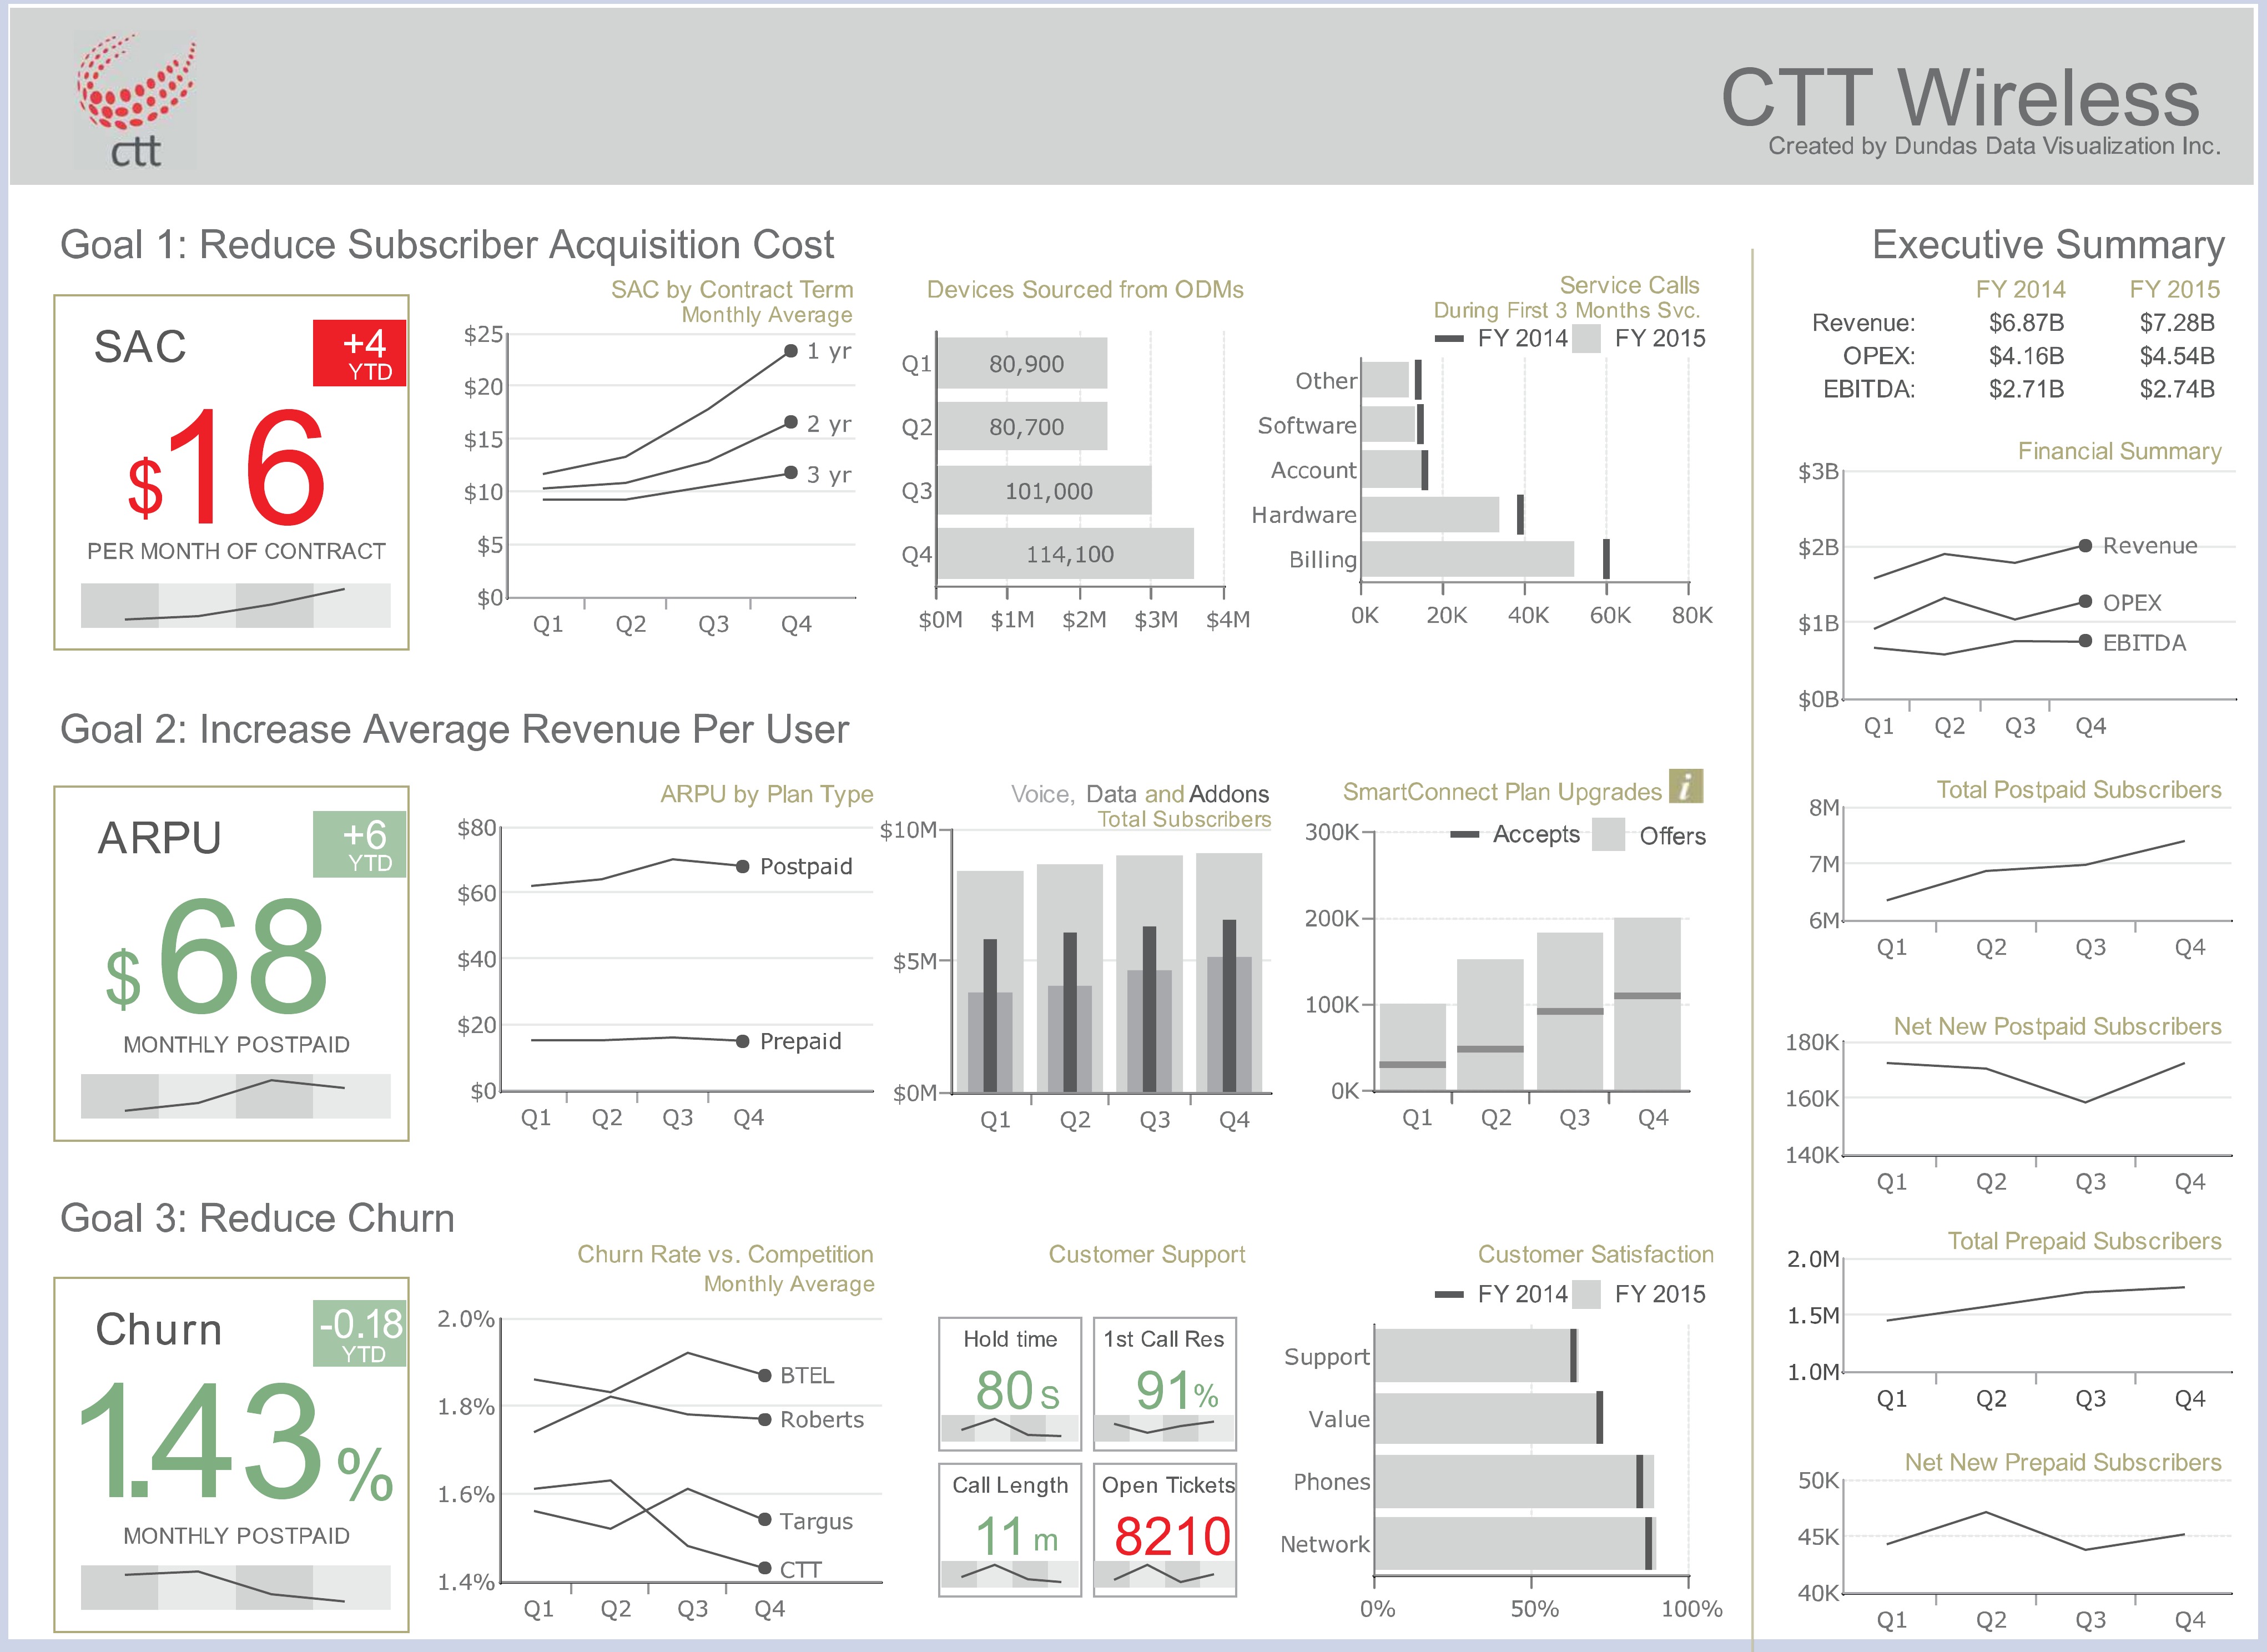
\includegraphics[width=\linewidth]{ch27_fig27_7_layout.png}
\end{center}
\end{column}
\end{columns}
\end{frame}

% =========================================================
\begin{frame}{Scenario and Business Context}
\twocol{
\begin{block}{Who uses it?}
\begin{itemize}
  \item Executives and senior management at a telecom company.
  \item Used in management, board, or stakeholder meetings.
  \item The goal is executive-level monitoring, not deep interactive analysis.
\end{itemize}
\end{block}
\begin{block}{What must it answer quickly?}
\begin{itemize}
  \item Is the company on track against strategic goals?
  \item Which metrics are improving or worsening?
\end{itemize}
\end{block}
}{
\begin{center}
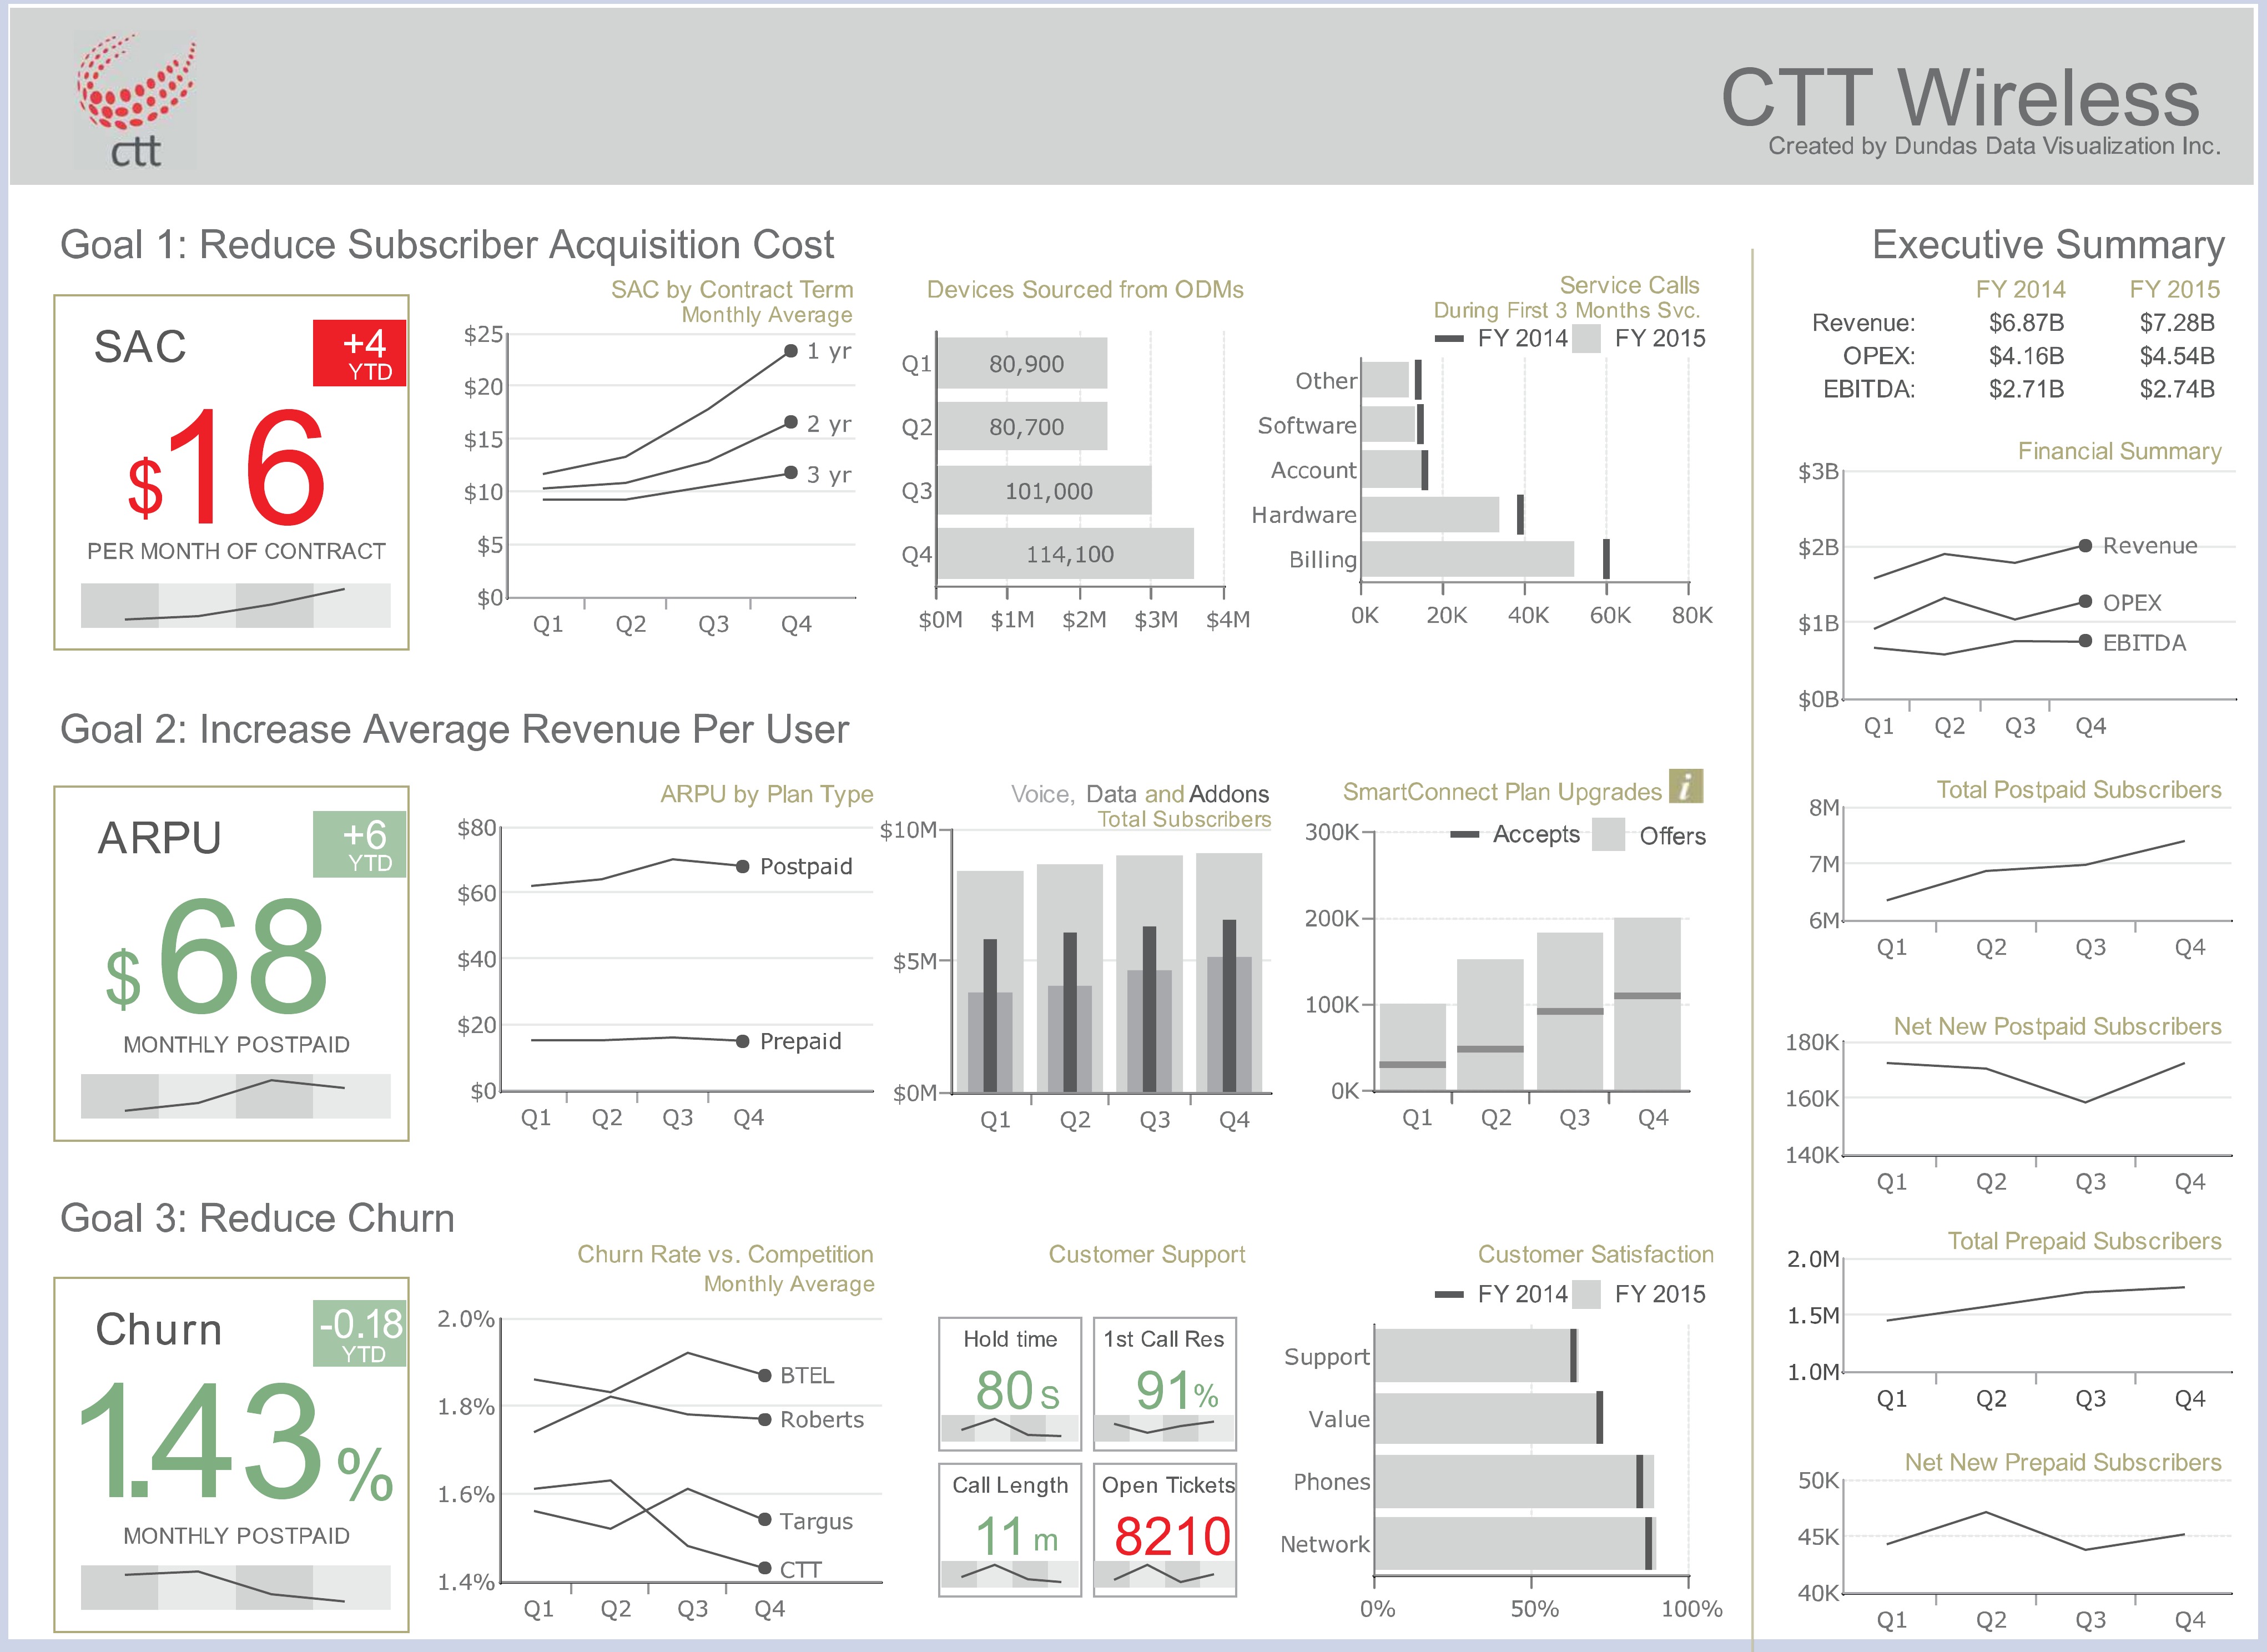
\includegraphics[width=\linewidth,height=0.55\textheight,keepaspectratio]{ch27_fig27_7_layout.png}
\end{center}
}
\keymessage{Use this as a monitoring view: status first, diagnosis second.}
\end{frame}

% =========================================================
\begin{frame}{Dashboard Design Logic}
\begin{center}
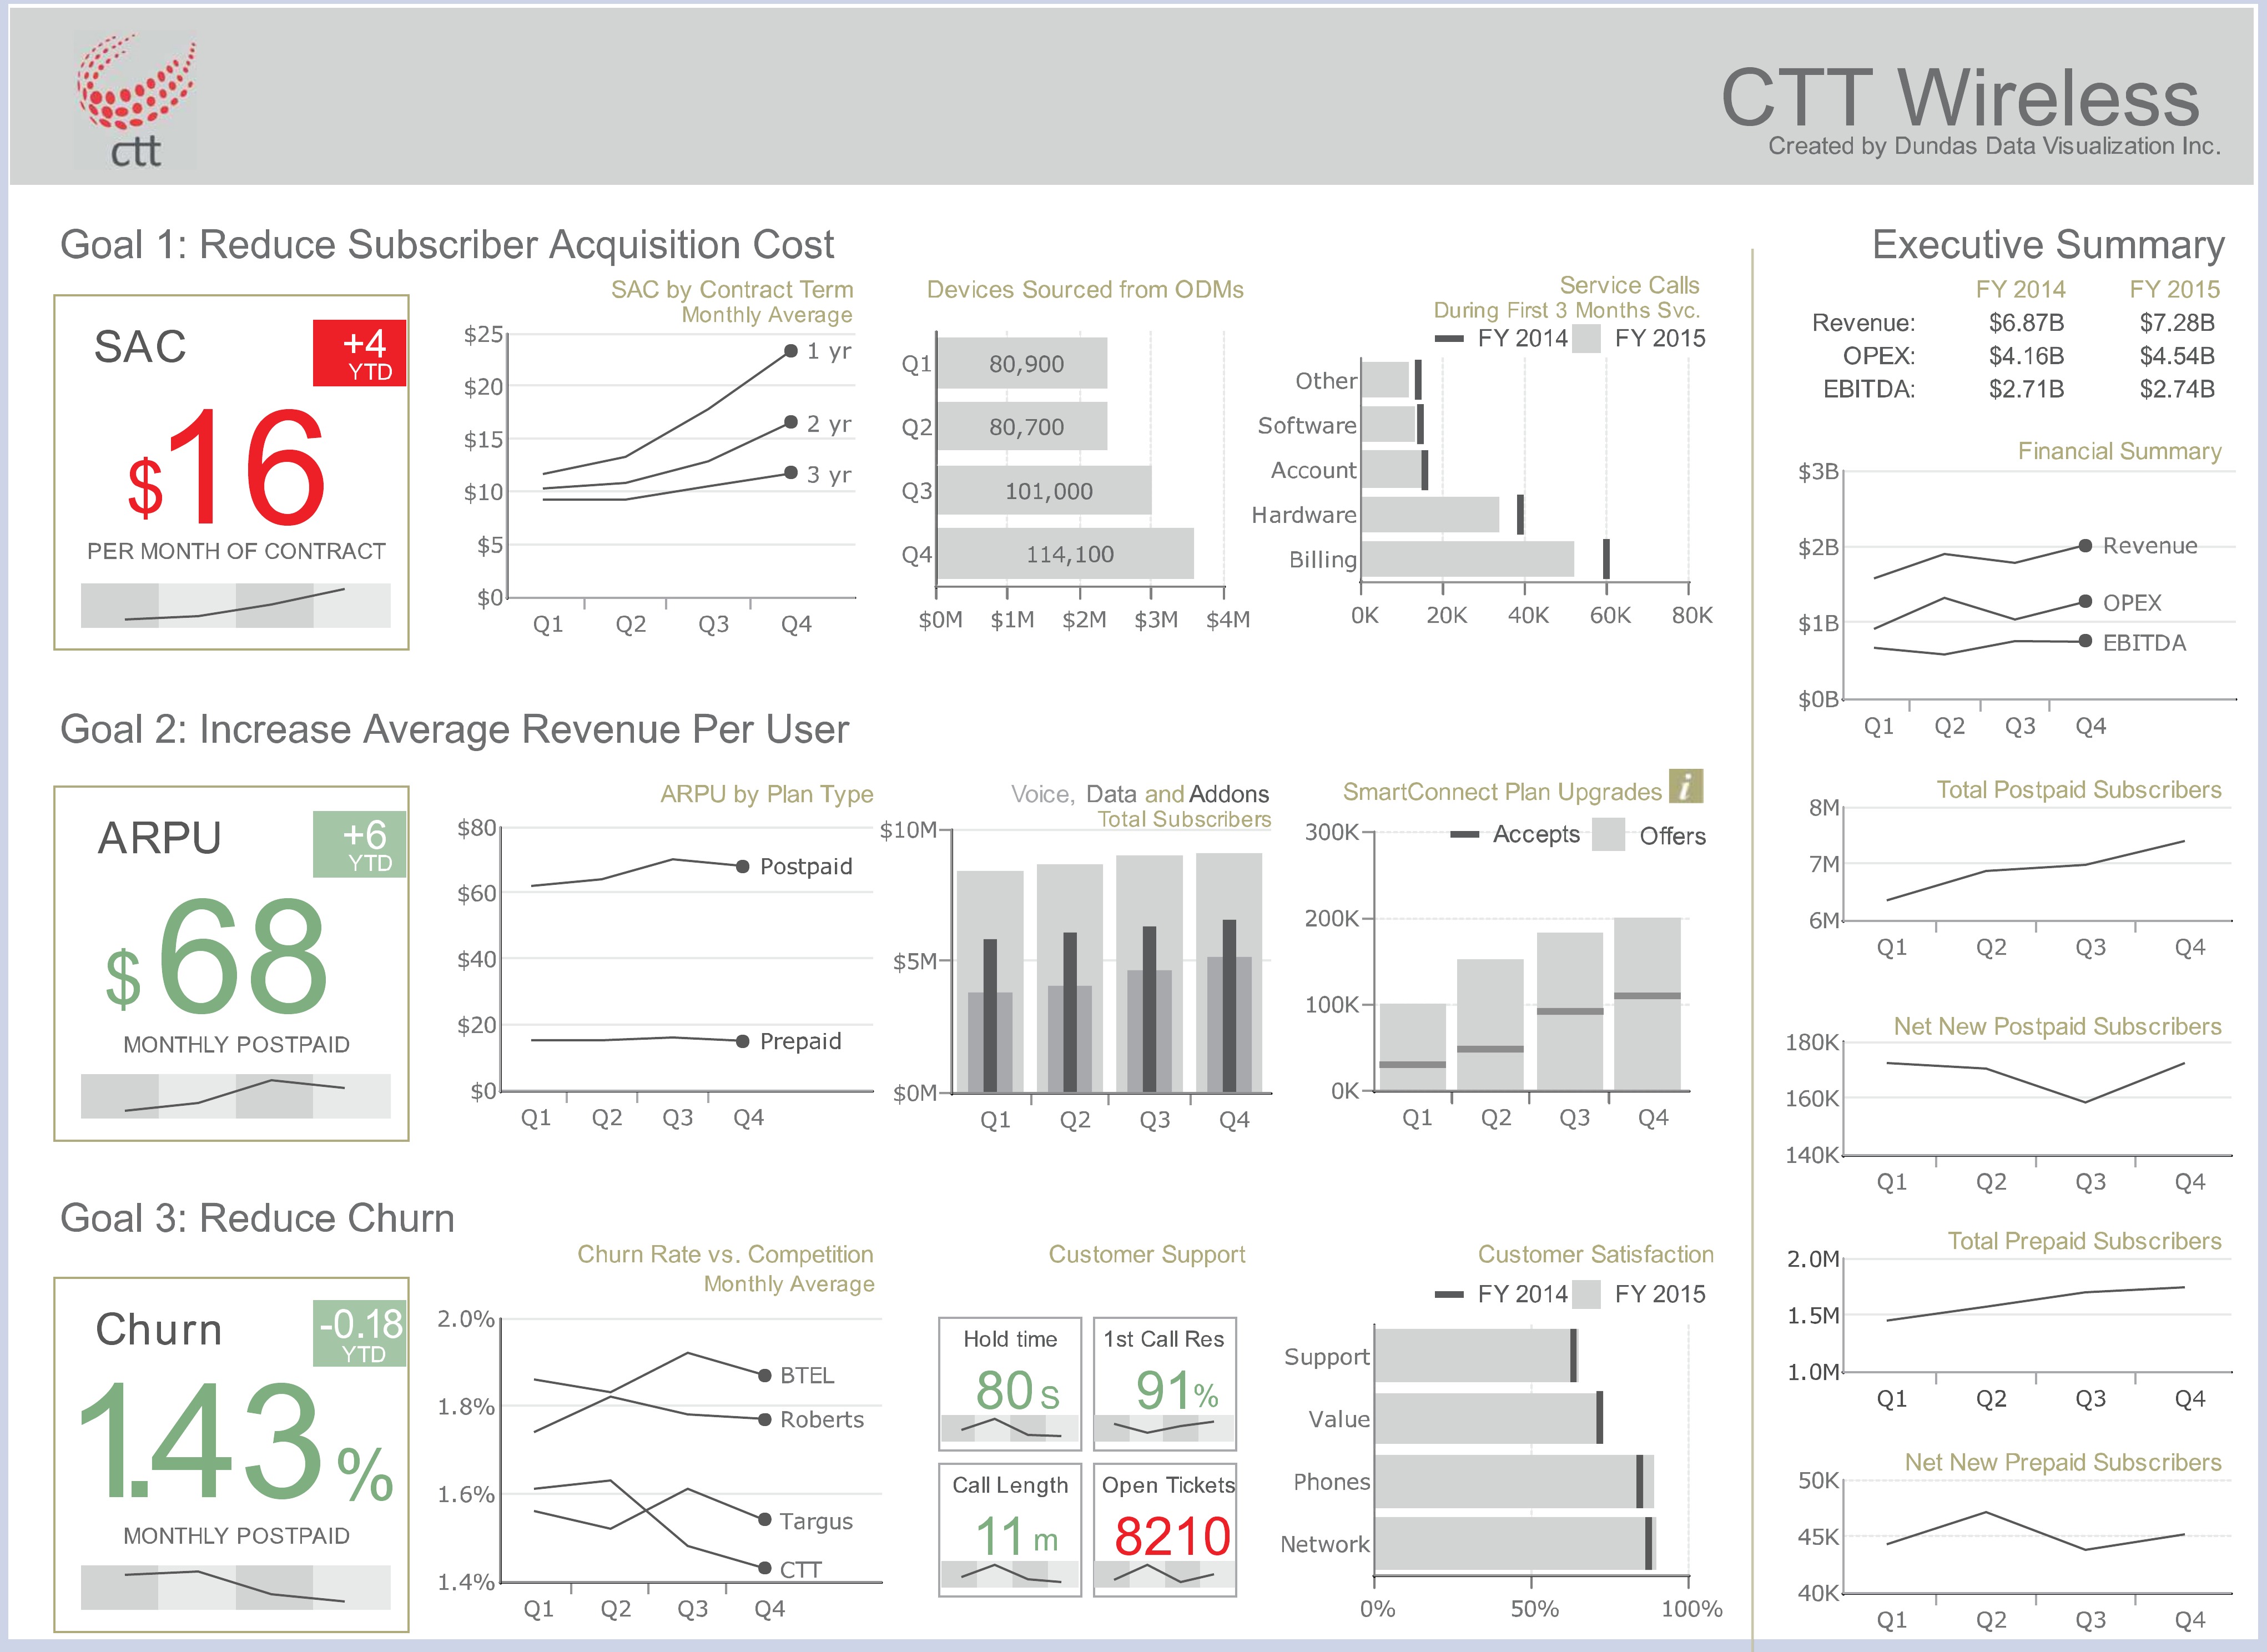
\includegraphics[width=0.95\linewidth,height=0.50\textheight,keepaspectratio]{ch27_fig27_7_layout.png}
\end{center}
\vspace{-2pt}
\begin{block}{The dashboard is structured around four information zones}
\begin{itemize}
  \item Row 1: \keyterm{Reduce Subscriber Acquisition Cost}.
  \item Row 2: \keyterm{Increase Average Revenue Per User}.
  \item Row 3: \keyterm{Reduce Churn}.
  \item Right column: \keyterm{Executive Summary} for finance and subscriber status.
\end{itemize}
\end{block}
\end{frame}

% =========================================================
\begin{frame}{Goal 1: Reduce SAC}
\begin{center}
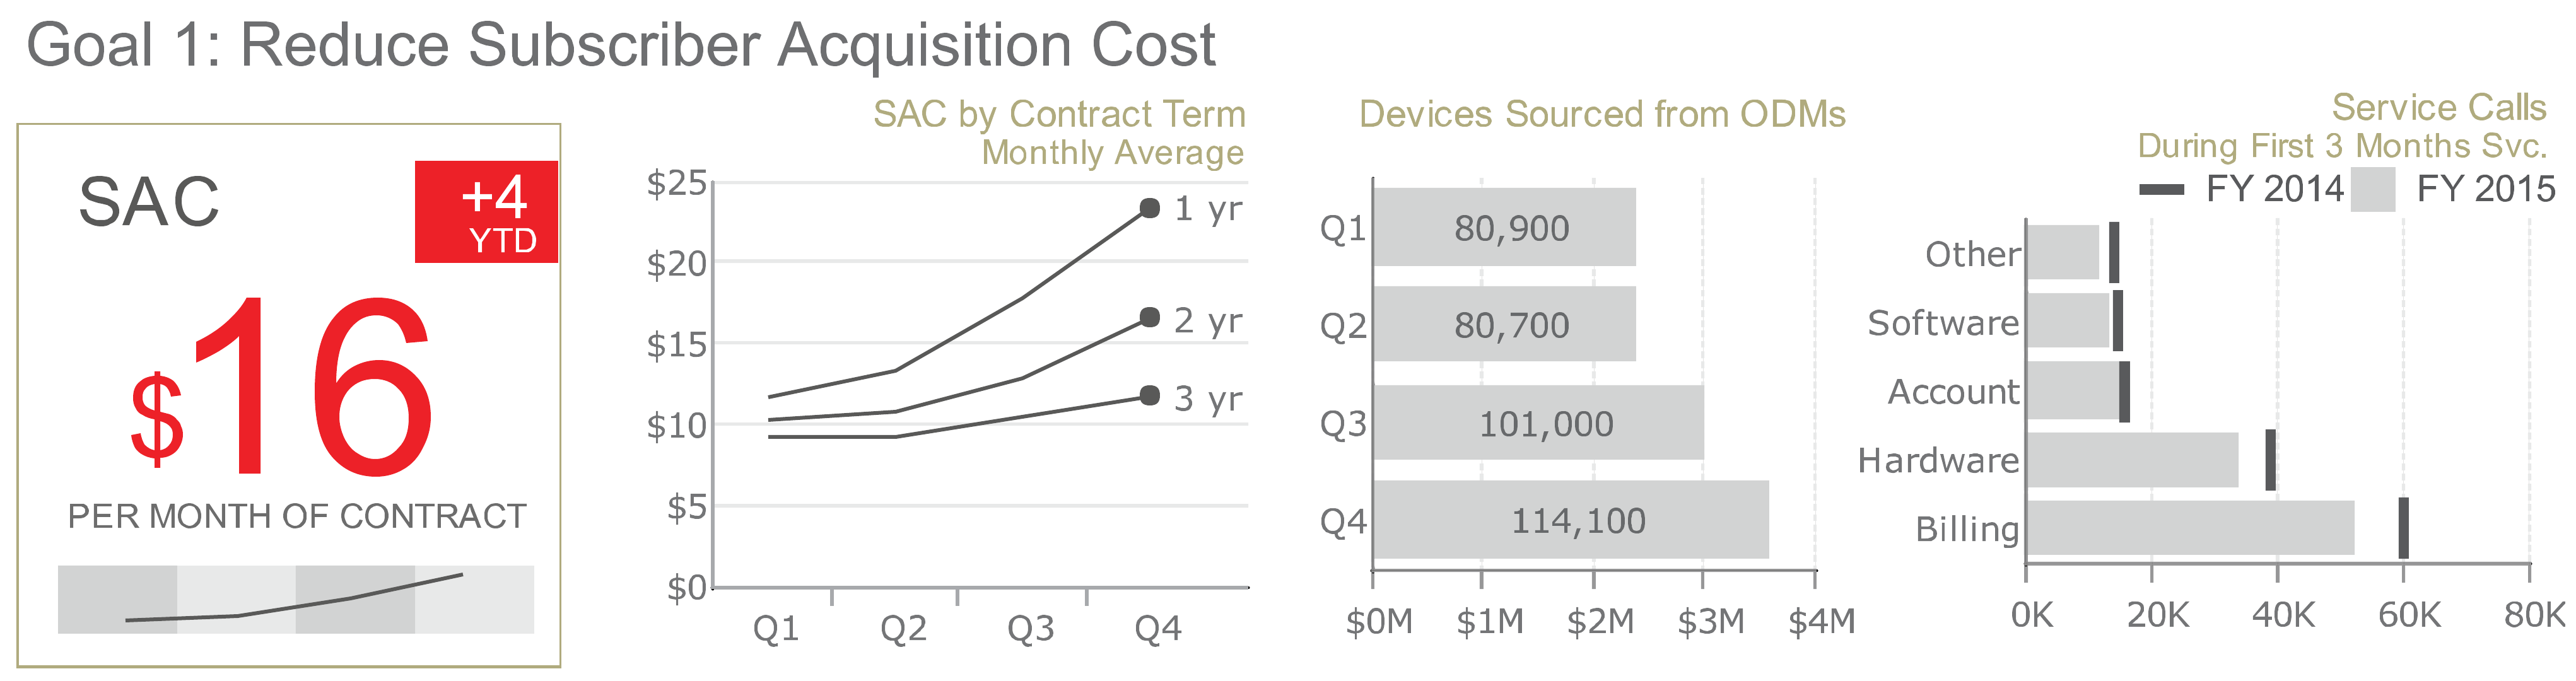
\includegraphics[width=\linewidth,height=0.43\textheight,keepaspectratio]{ch27_fig27_1_sac.png}
\end{center}
\vspace{-0.10cm}
\noindent
\begin{minipage}[t]{0.30\textwidth}
\goalcard{Status}{\cardline{\bad{\$16}/month of contract.}\cardline{\bad{+4 YTD} above benchmark.}}
\end{minipage}\hfill
\begin{minipage}[t]{0.30\textwidth}
\goalcard{Drivers}{\cardline{Contract term changes cost.}\cardline{ODM device mix adds pressure.}}
\end{minipage}\hfill
\begin{minipage}[t]{0.30\textwidth}
\goalcard{Operational signal}{\cardline{Service calls show burden.}\cardline{Target lines show FY2014 gap.}}
\end{minipage}
\keymessage{Priority: identify which acquisition driver is pushing SAC above the benchmark.}
\end{frame}

% =========================================================
\begin{frame}{Goal 2: Increase ARPU}
\begin{center}
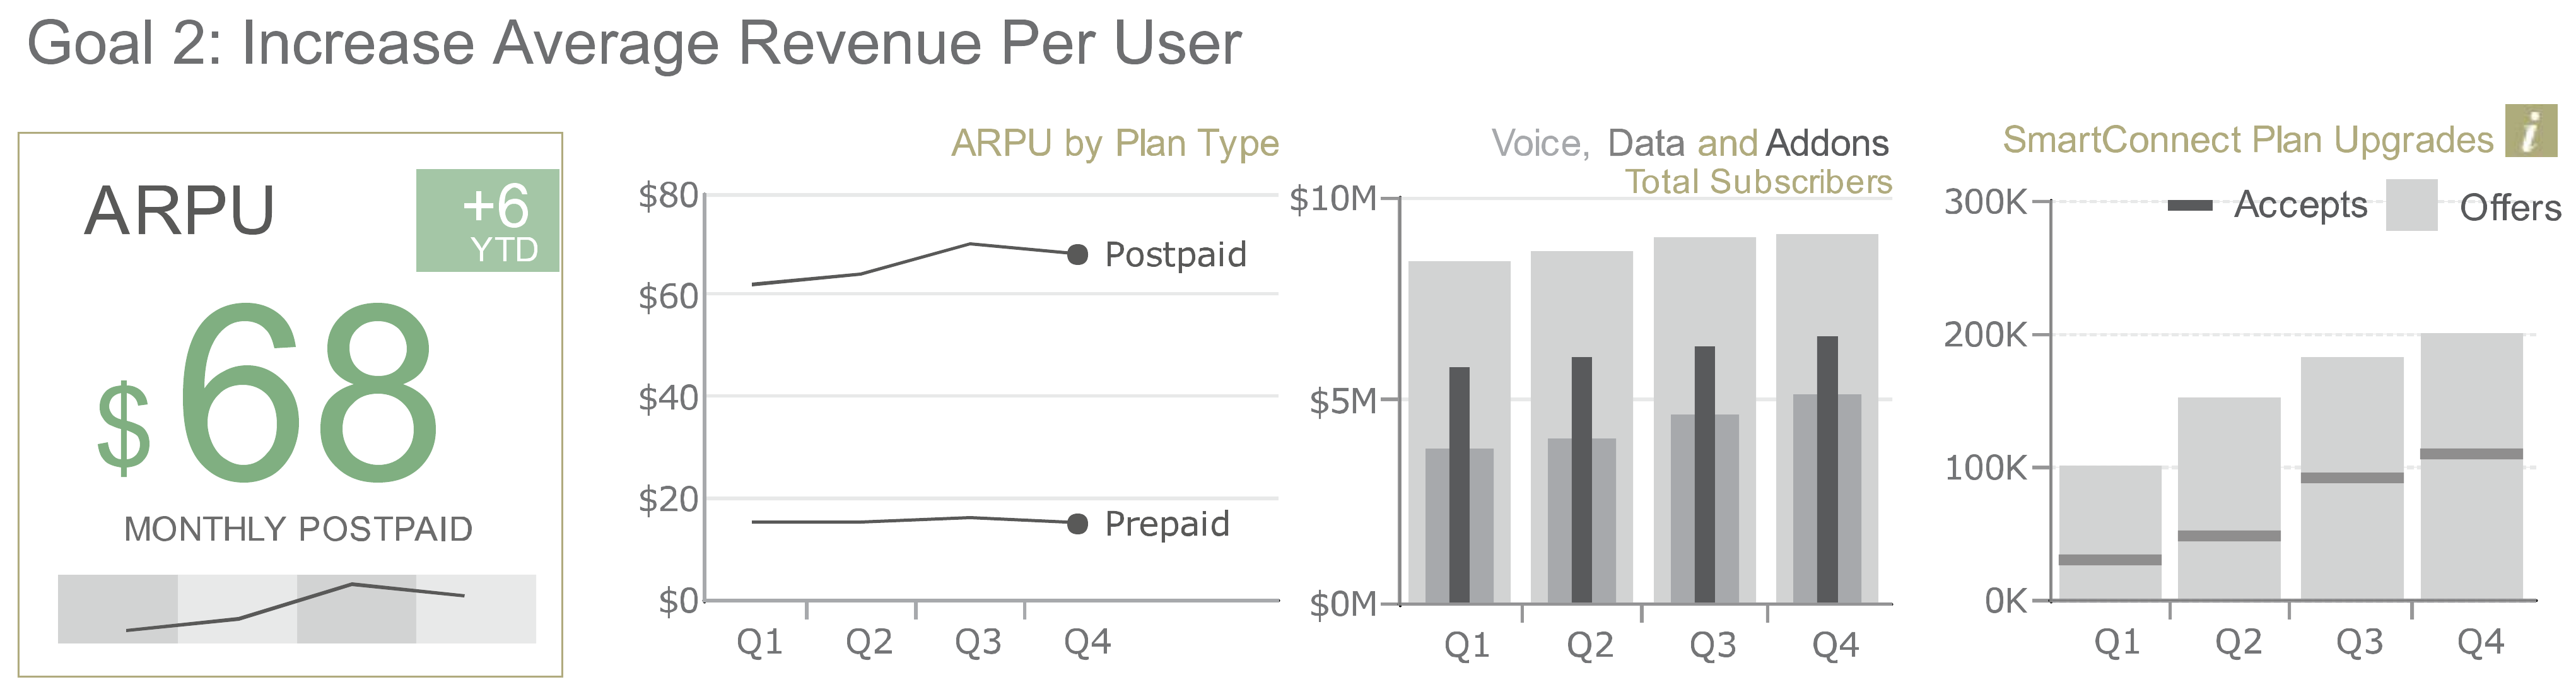
\includegraphics[width=\linewidth,height=0.43\textheight,keepaspectratio]{ch27_fig27_2_arpu.png}
\end{center}
\vspace{-0.10cm}
\noindent
\begin{minipage}[t]{0.30\textwidth}
\goalcard{Status}{\cardline{\good{\$68} monthly postpaid.}\cardline{\good{+6 YTD} revenue lift.}}
\end{minipage}\hfill
\begin{minipage}[t]{0.30\textwidth}
\goalcard{Revenue mix}{\cardline{Postpaid/prepaid split.}\cardline{Add-ons show contribution.}}
\end{minipage}\hfill
\begin{minipage}[t]{0.30\textwidth}
\goalcard{Conversion}{\cardline{Offers compared with accepts.}\cardline{Gaps show upgrade room.}}
\end{minipage}
\keymessage{Read ARPU growth through mix, add-on contribution, and upgrade acceptance.}
\end{frame}

% =========================================================
\begin{frame}{Goal 3: Reduce Churn}
\begin{center}
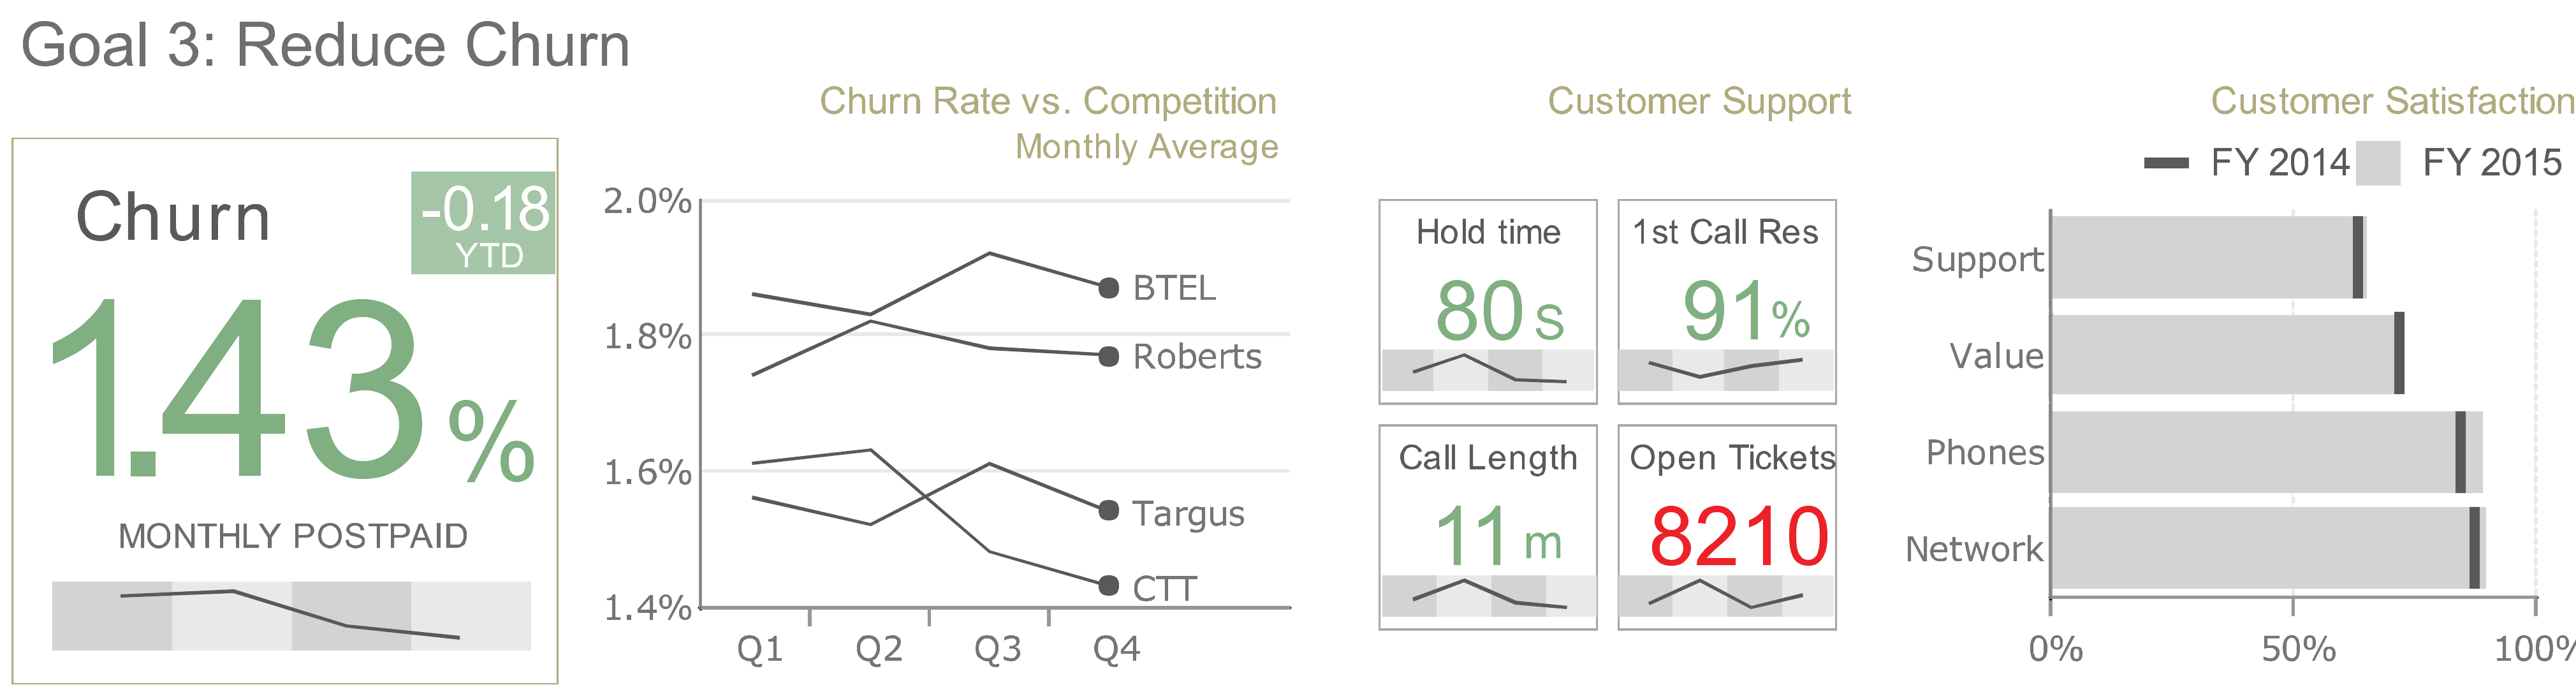
\includegraphics[width=\linewidth,height=0.43\textheight,keepaspectratio]{ch27_fig27_3_churn.png}
\end{center}
\vspace{-0.10cm}
\noindent
\begin{minipage}[t]{0.30\textwidth}
\goalcard{Status}{\cardline{\good{1.43\%} monthly churn.}\cardline{\good{-0.18 YTD} improvement.}}
\end{minipage}\hfill
\begin{minipage}[t]{0.30\textwidth}
\goalcard{Competitive view}{\cardline{CTT benchmarked vs peers.}\cardline{Direct labels avoid a legend.}}
\end{minipage}\hfill
\begin{minipage}[t]{0.30\textwidth}
\goalcard{Retention risk}{\cardline{Support KPIs show friction.}\cardline{Satisfaction flags churn risk.}}
\end{minipage}
\keymessage{The churn headline is favorable; support and satisfaction explain whether it is durable.}
\end{frame}

% =========================================================
\begin{frame}{Executive Summary}
\begin{columns}[T,onlytextwidth]
\begin{column}{0.38\textwidth}
\begin{center}
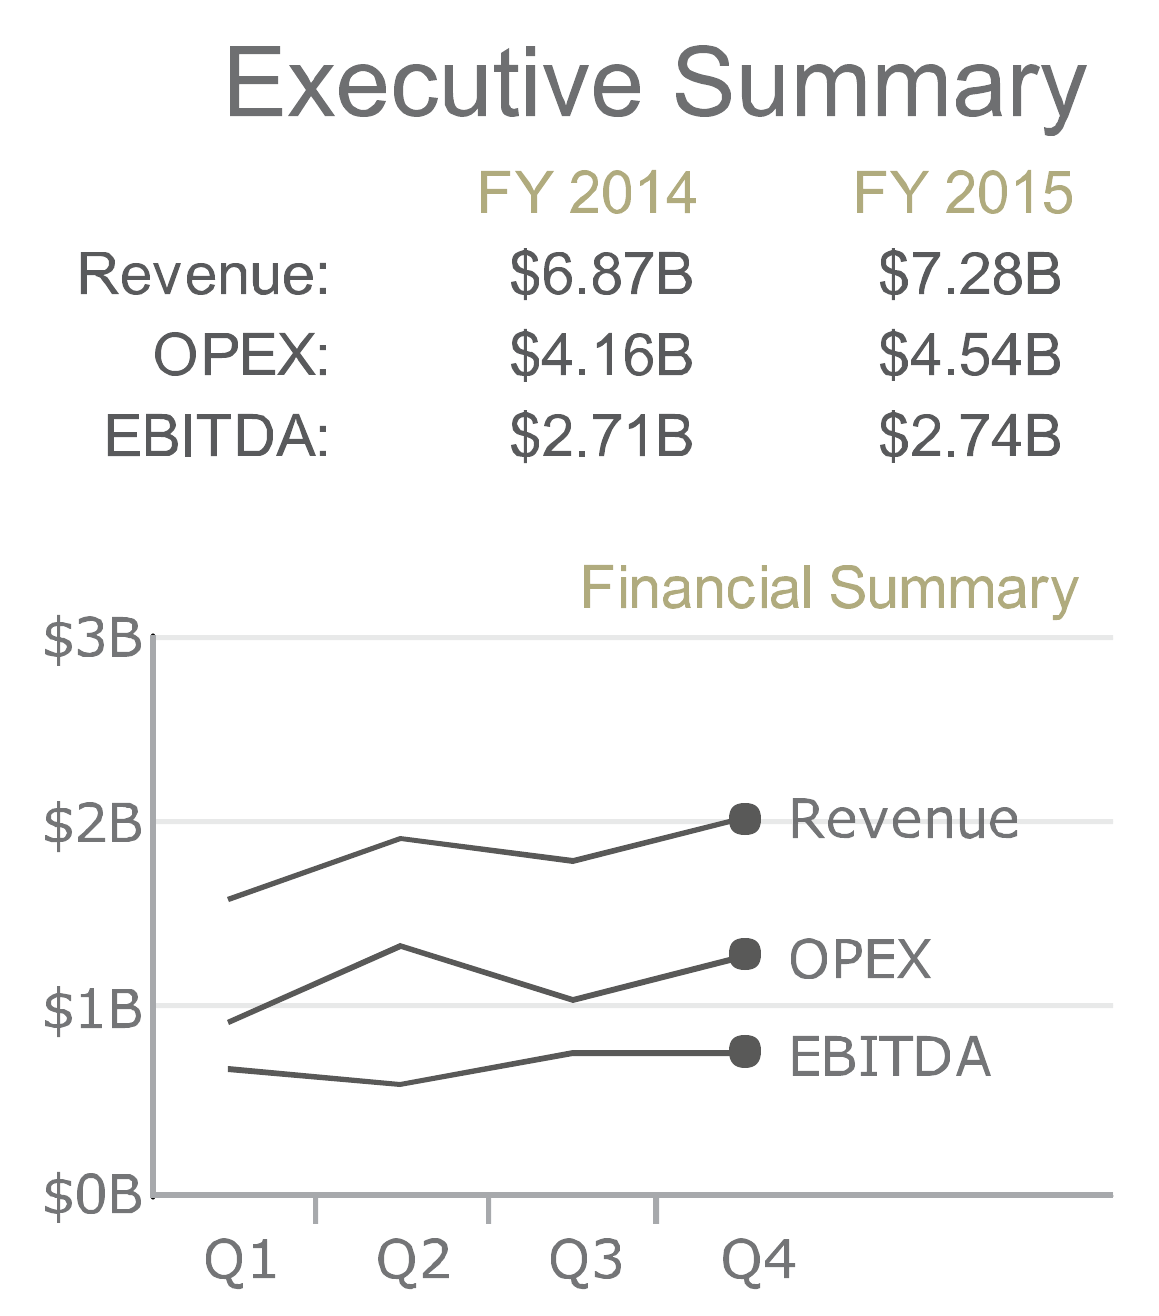
\includegraphics[width=\linewidth,height=0.52\textheight,keepaspectratio]{ch27_fig27_4_exec_financial_trim.png}\\[0.08cm]
\scriptsize\textbf{Finance:} revenue, OPEX, and EBITDA stay visible as executive context.
\end{center}
\end{column}
\begin{column}{0.36\textwidth}
\begin{center}
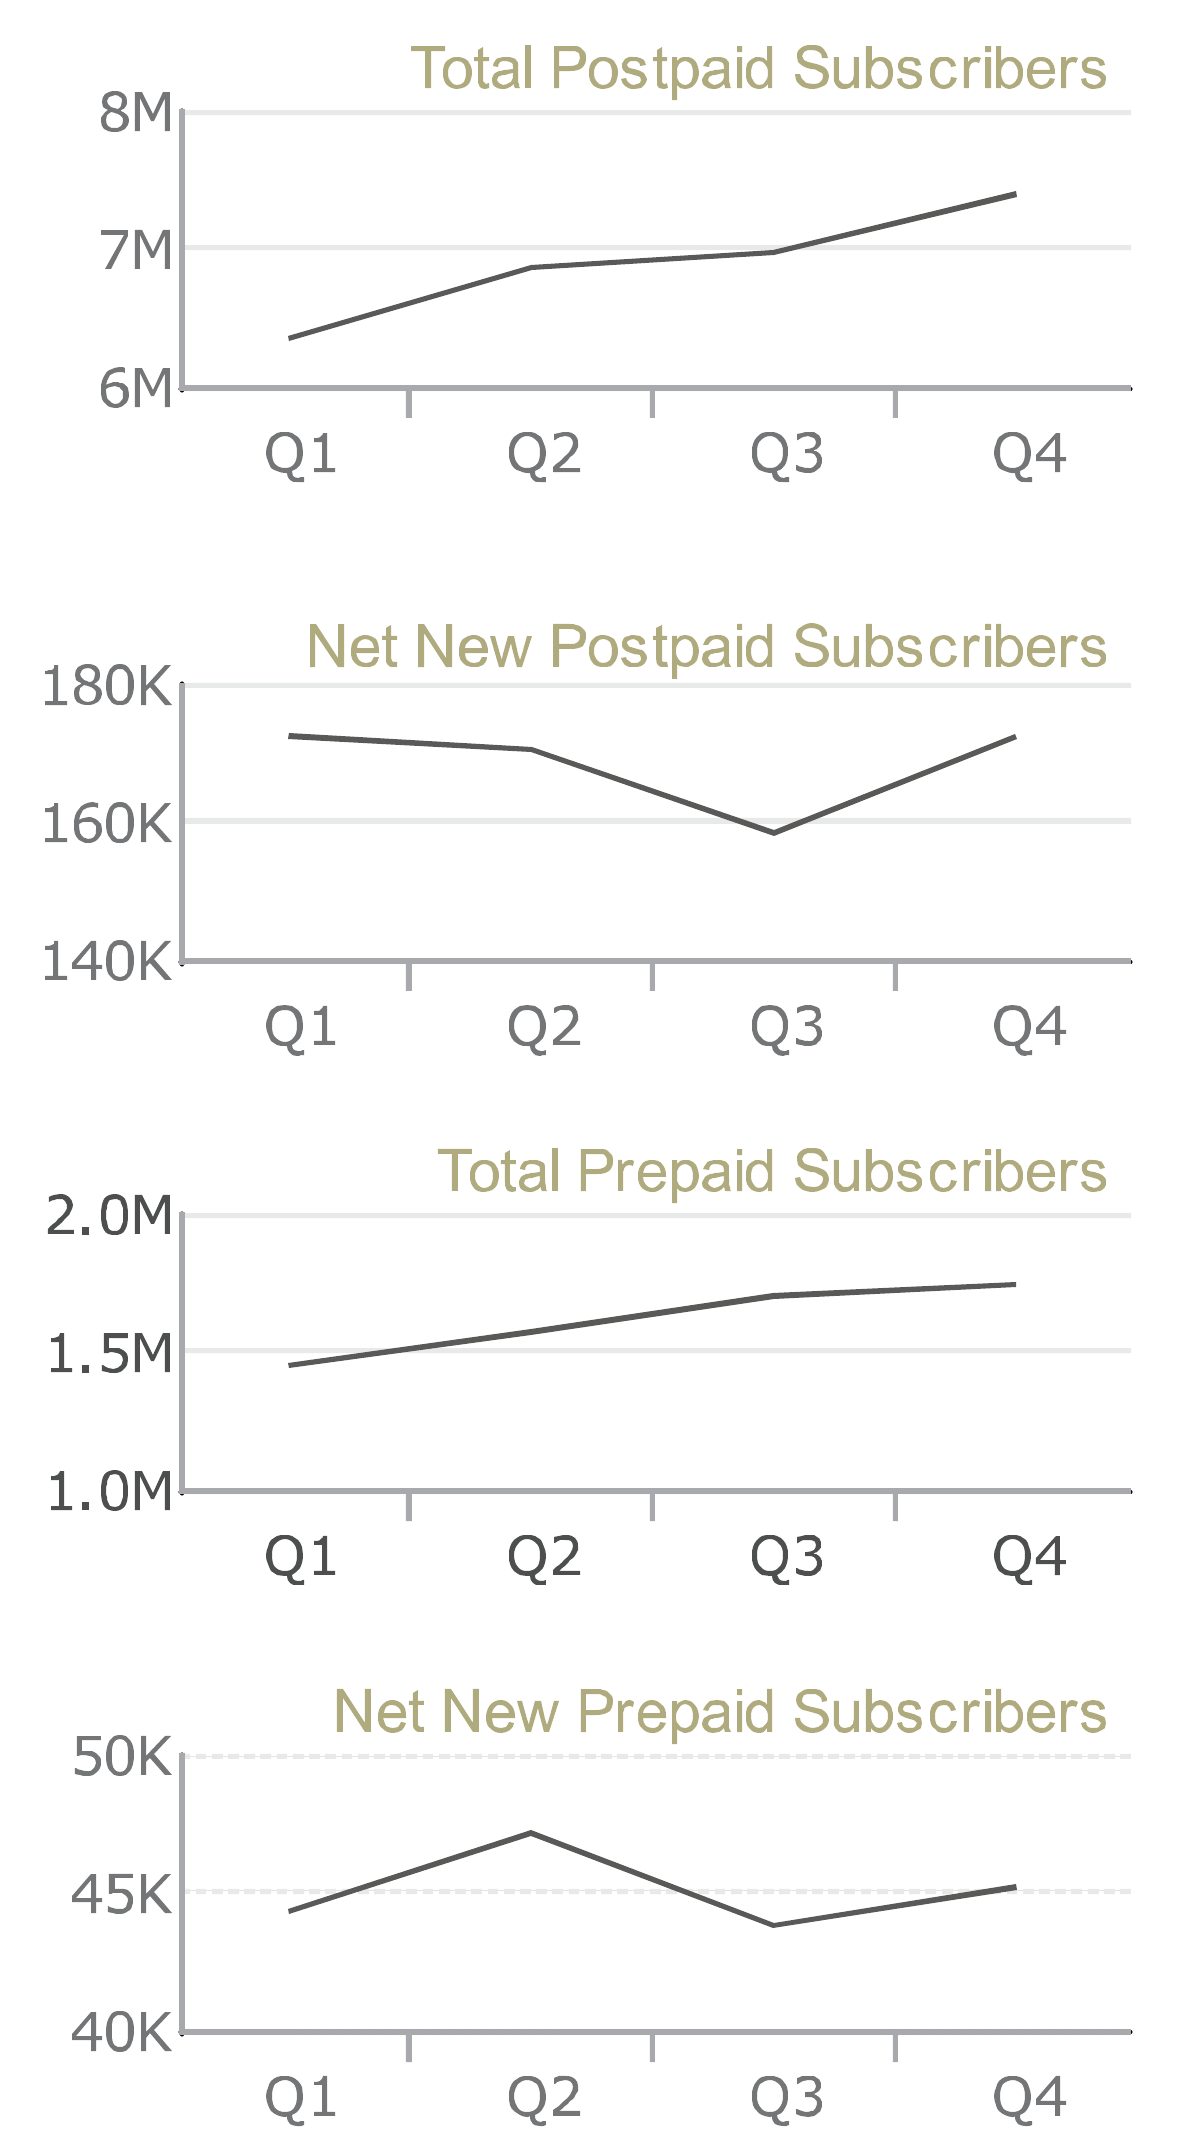
\includegraphics[height=0.68\textheight,keepaspectratio]{ch27_fig27_4_exec_subscribers_trim.png}
\end{center}
\end{column}
\begin{column}{0.22\textwidth}
\footnotesize
\textcolor{cttBlue}{\textbf{Executive read}}\\[-0.02cm]
\textcolor{cttBlue}{\rule{\linewidth}{0.6pt}}
\vspace{0.08cm}

\begin{tabular}{@{}p{0.13\linewidth}@{\hspace{0.05cm}}p{0.70\linewidth}@{}}
\textcolor{cttBlue}{\textbf{01}} & Financial health\\[0.13cm]
\textcolor{cttBlue}{\textbf{02}} & Subscriber base\\[0.13cm]
\textcolor{cttBlue}{\textbf{03}} & Net additions
\end{tabular}

\vspace{0.24cm}
\scriptsize
\textbf{Use:} company context for the three goal rows.\\[0.10cm]
\textbf{Do not use:} detailed diagnosis by itself.
\end{column}
\end{columns}
\keymessage{The summary column gives context; the goal rows explain what to act on.}
\end{frame}

% =========================================================
\begin{frame}{Why This Works: Compact but Informative}
\begin{columns}[T,onlytextwidth]
\begin{column}{0.58\textwidth}
\begin{center}
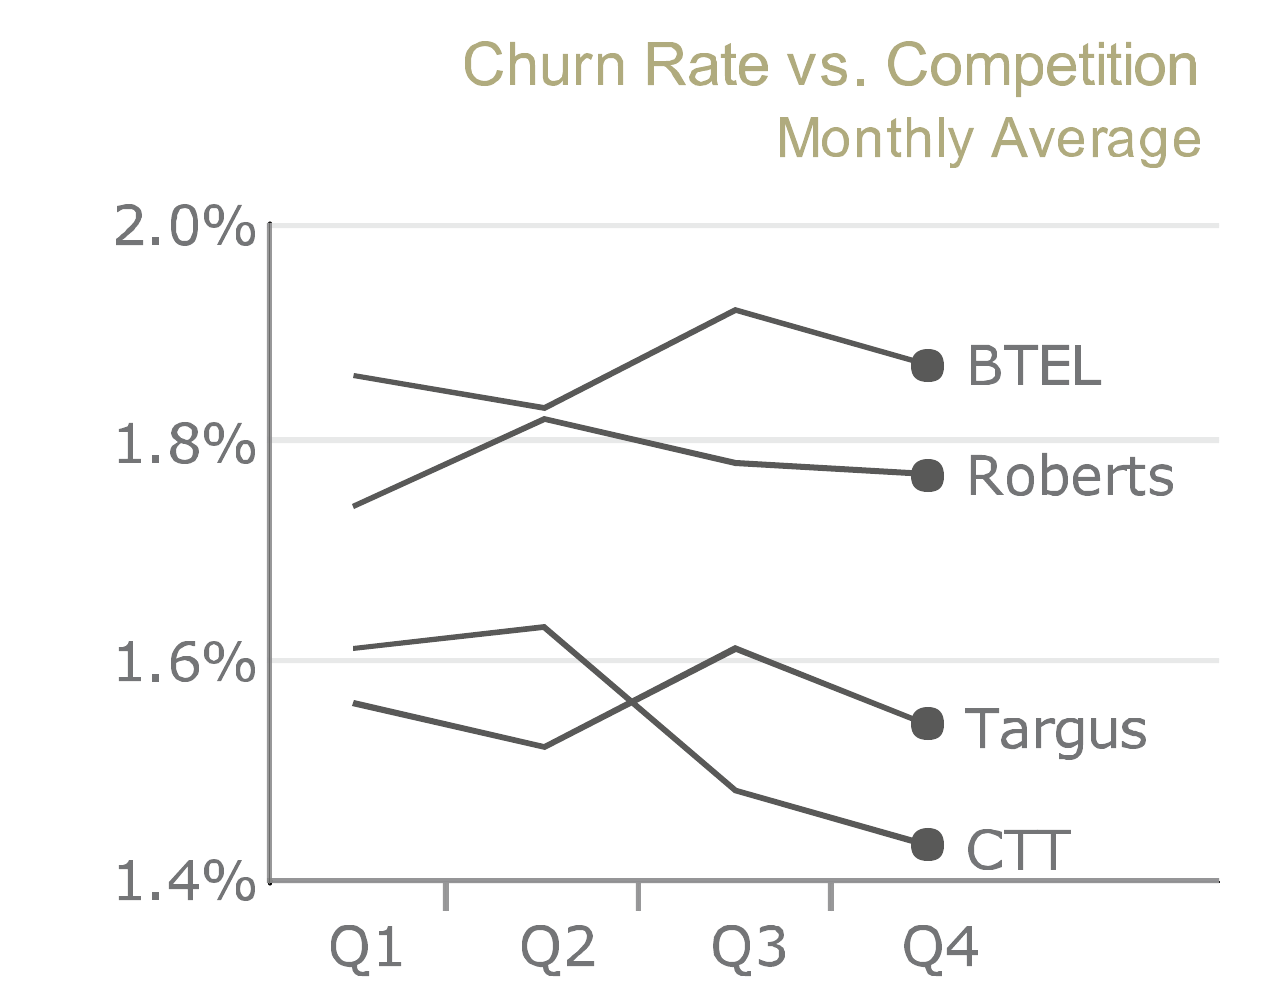
\includegraphics[width=\linewidth,height=0.53\textheight,keepaspectratio]{ch27_fig27_5_direct_labels.png}
\end{center}
\footnotesize\textbf{Direct labels.} Line-end labels remove the legend lookup and keep each series attached to its endpoint.
\end{column}
\begin{column}{0.38\textwidth}
\begin{center}
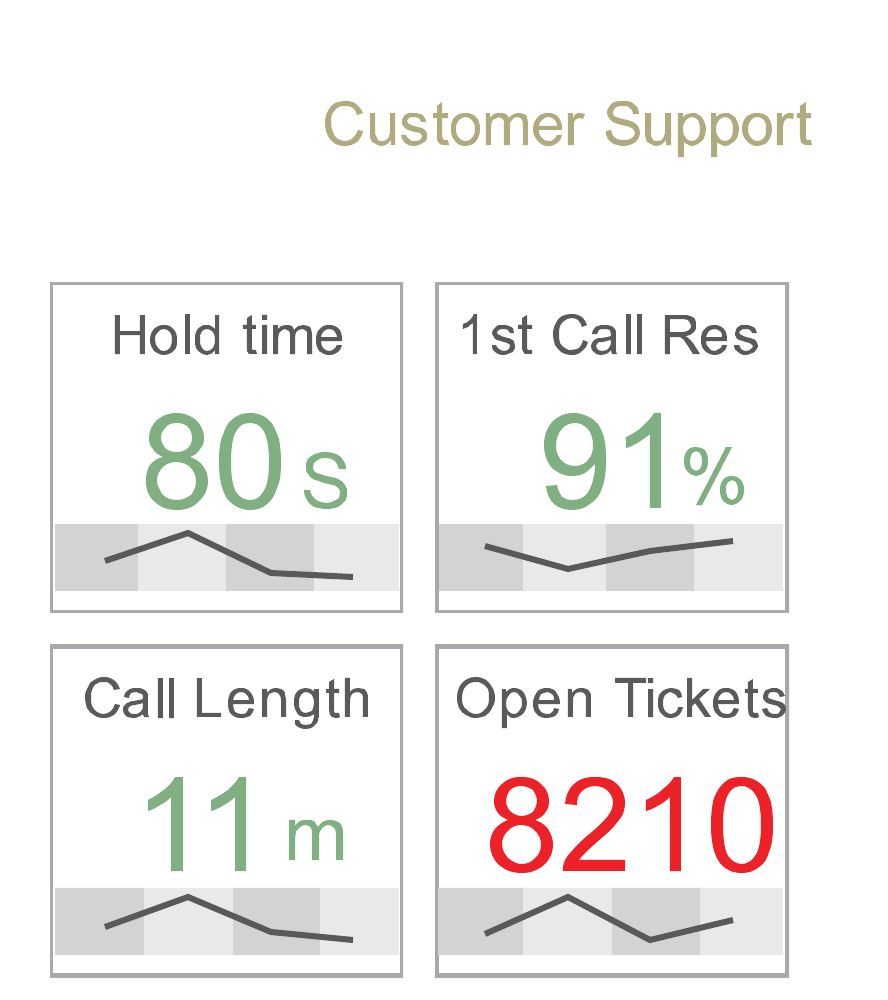
\includegraphics[width=0.82\linewidth,height=0.53\textheight,keepaspectratio]{ch27_fig27_6_customer_support.png}
\end{center}
\footnotesize\textbf{Small KPI cards.} Sparklines add trend context while keeping four support measures in a tight space.
\end{column}
\end{columns}
\keymessage{Compact visuals work when labels, trends, and comparisons are resolved inside the chart.}
\end{frame}

% =========================================================
\begin{frame}{Layout Supports Quick Reading}
\twocol{
\begin{block}{Design principles used}
\begin{itemize}
  \item \keyterm{Proximity}: related charts are placed near one another.
  \item \keyterm{Closure}: each goal is perceived as a separate group.
  \item \keyterm{Alignment}: rows and columns make scanning predictable.
  \item \keyterm{Visual hierarchy}: KPI cards appear first, summary stays on the right.
\end{itemize}
\end{block}
\vspace{-0.03cm}
\footnotesize\textbf{Reading paths:} scan horizontally to analyze one goal; scan the right column for company-wide status.
}{
\begin{center}
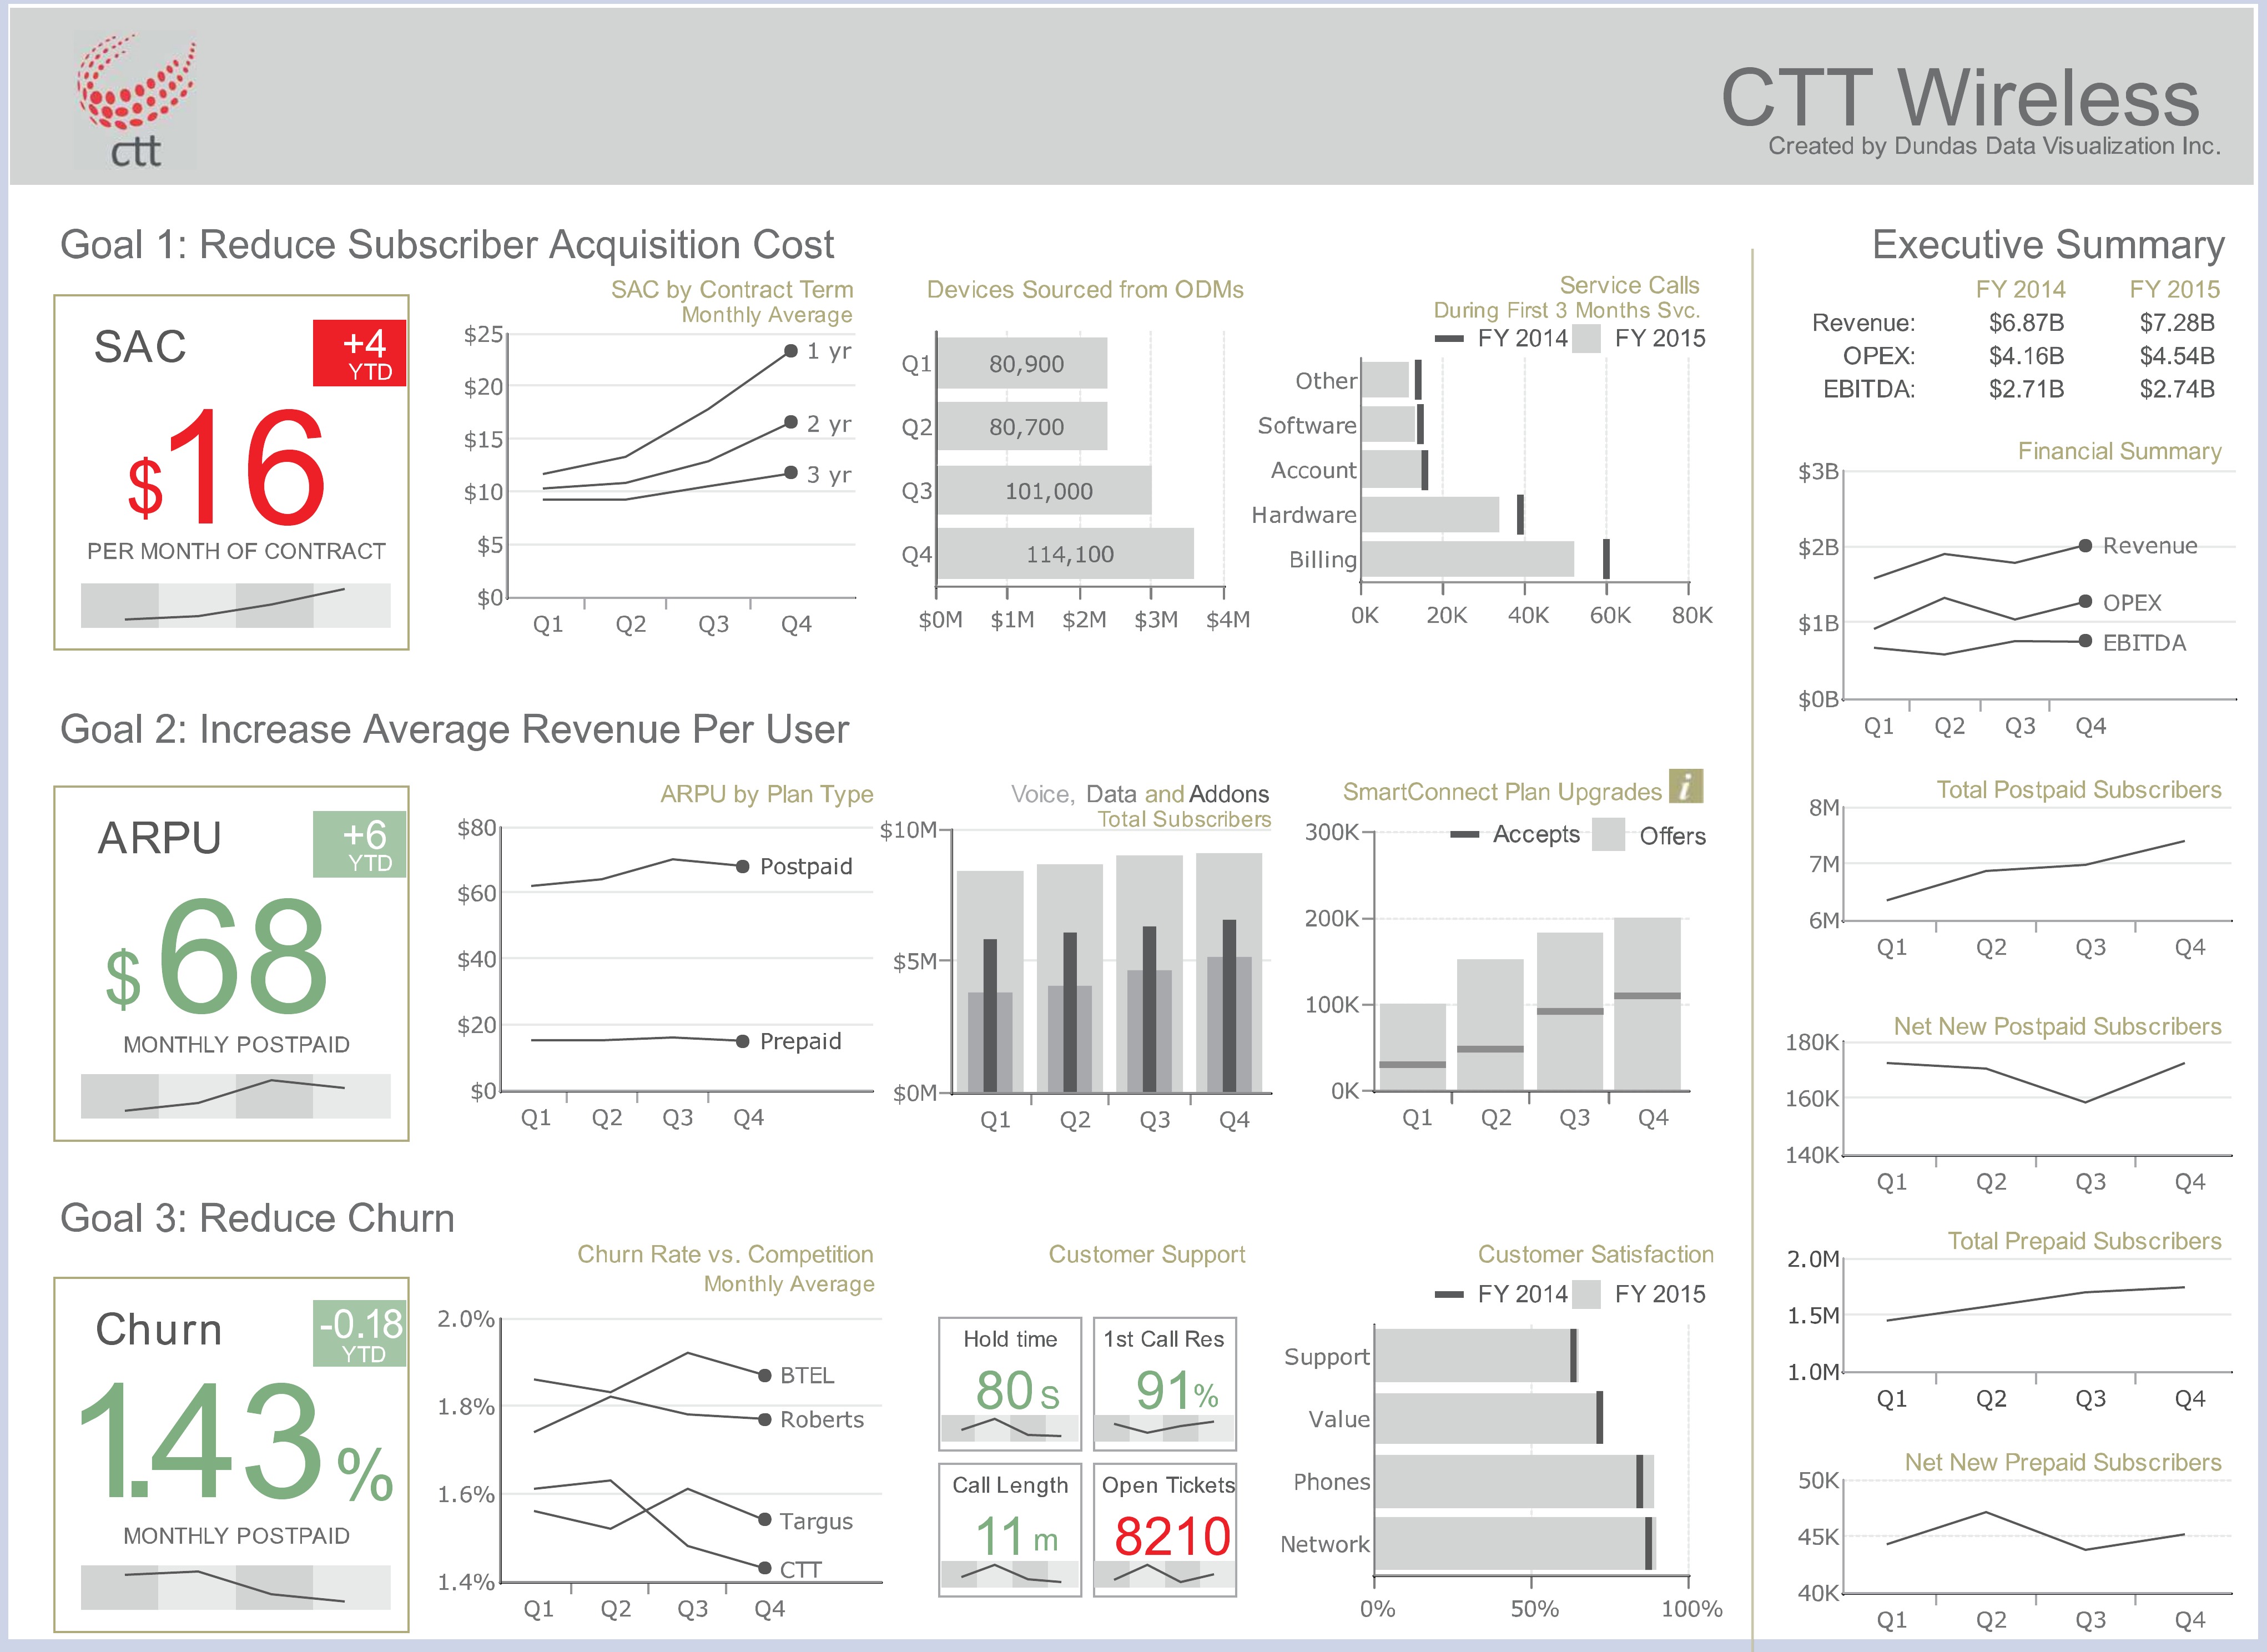
\includegraphics[width=\linewidth,height=0.54\textheight,keepaspectratio]{ch27_fig27_7_layout.png}
\end{center}
}
\keymessage{The layout supports two reading paths: across each goal row, then down the summary column.}
\end{frame}

% =========================================================
\begin{frame}{Chart Type Selection}
\begin{columns}[T,onlytextwidth]
\begin{column}{0.66\textwidth}
\begin{center}
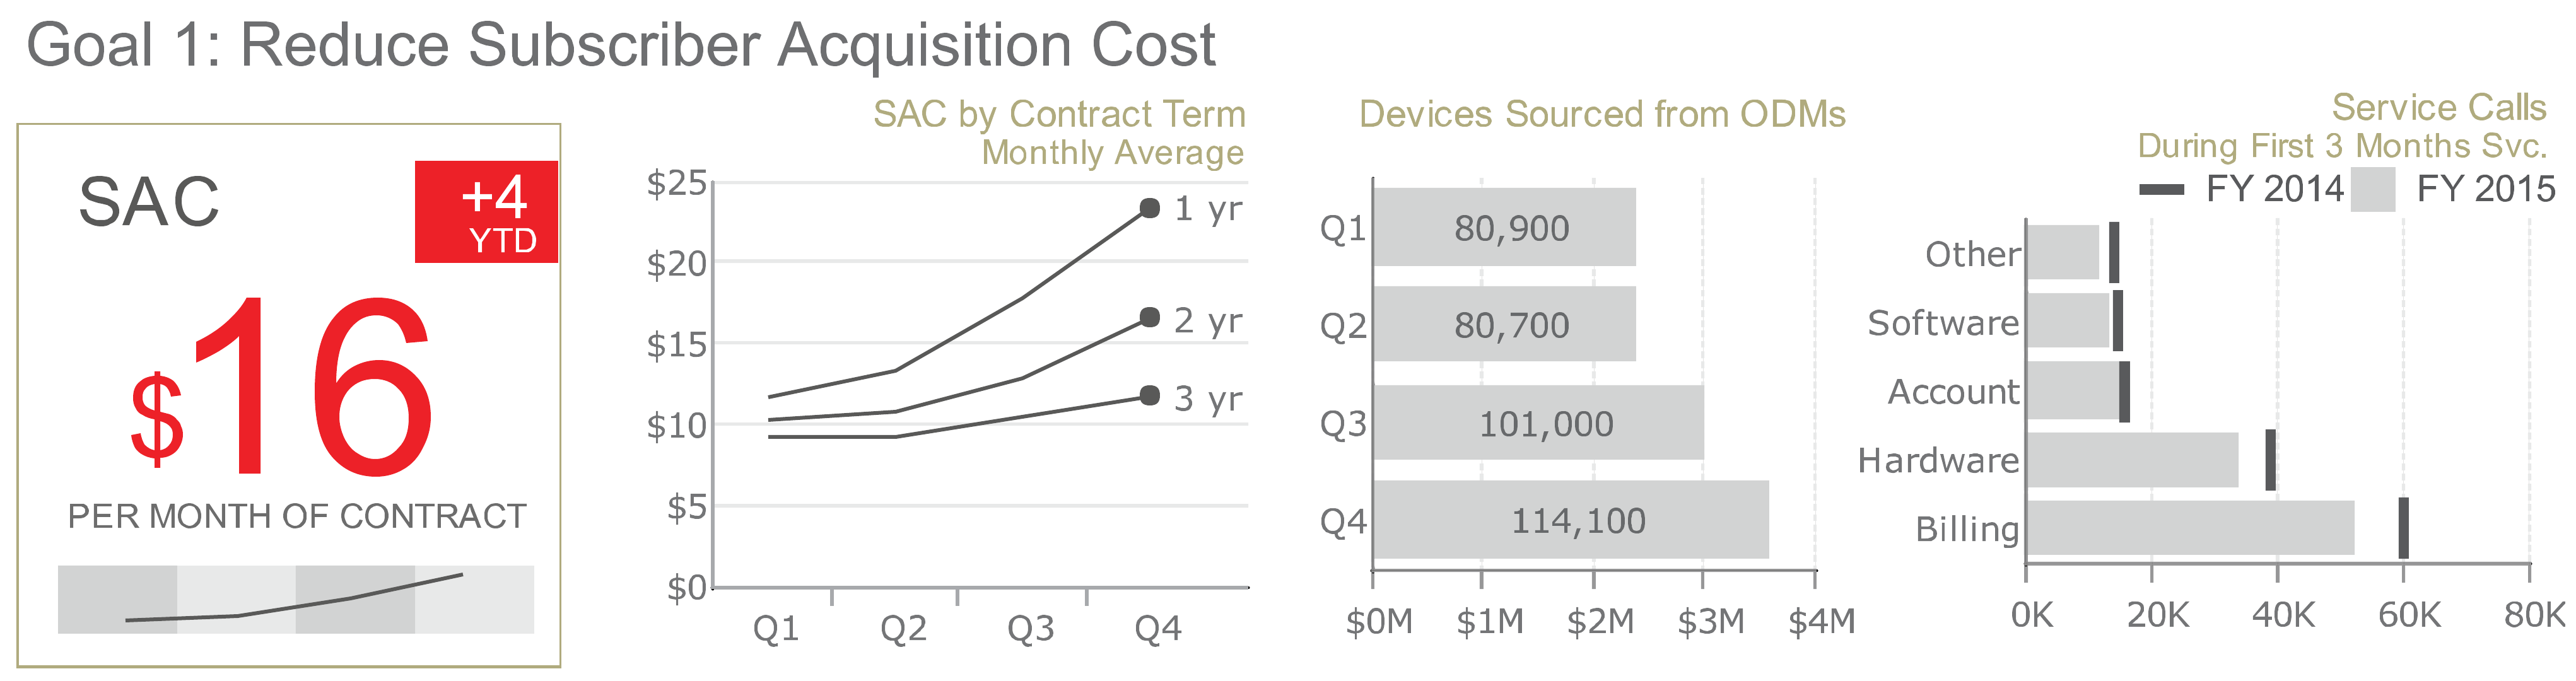
\includegraphics[width=\linewidth,height=0.40\textheight,keepaspectratio]{ch27_fig27_1_sac.png}
\end{center}
\footnotesize
\textbf{Goal row:} KPI card, trend line, comparison bars, and target line are read as one decision unit.
\end{column}
\begin{column}{0.30\textwidth}
\begin{center}
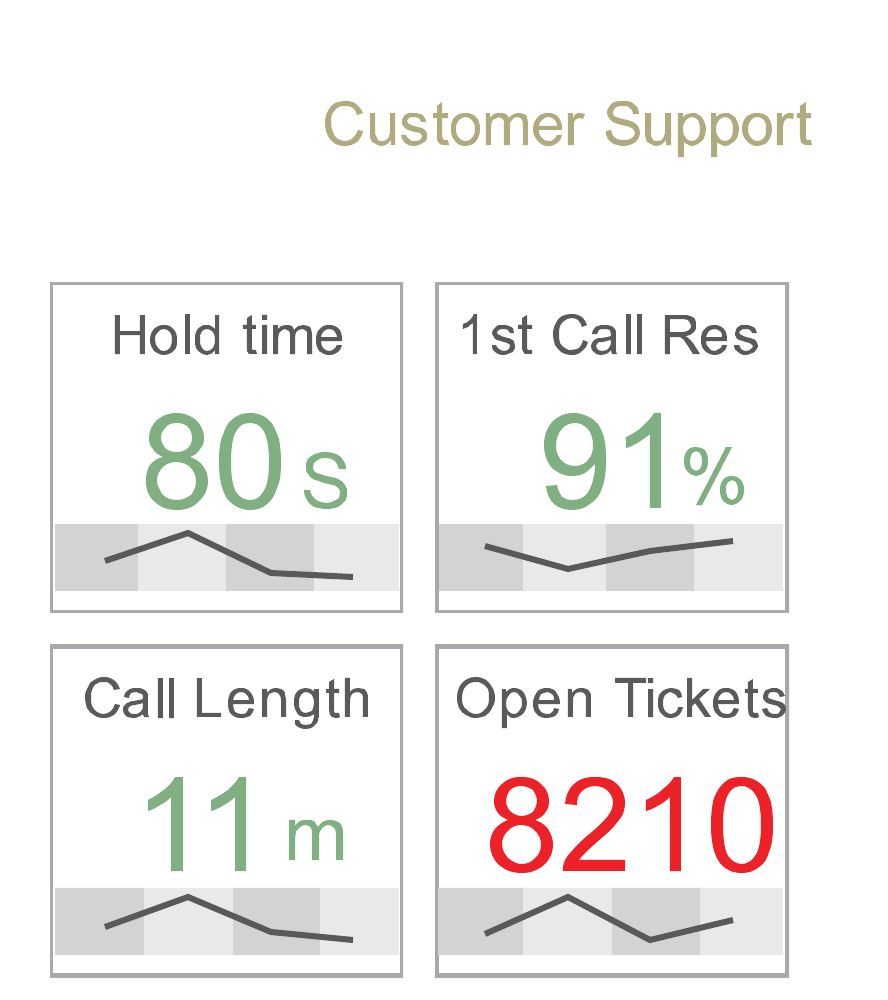
\includegraphics[width=0.78\linewidth,height=0.34\textheight,keepaspectratio]{ch27_fig27_6_customer_support.png}
\end{center}
\footnotesize
\textbf{KPI cards:} sparklines provide compact trend context without opening a separate chart.
\end{column}
\end{columns}
\vspace{0.10cm}
\noindent
\begin{minipage}[t]{0.23\textwidth}
\footnotesize\keyterm{Line charts}\\[-0.02cm]
\scriptsize Trends over time.
\end{minipage}\hfill
\begin{minipage}[t]{0.23\textwidth}
\footnotesize\keyterm{Bar charts}\\[-0.02cm]
\scriptsize Category and target comparisons.
\end{minipage}\hfill
\begin{minipage}[t]{0.23\textwidth}
\footnotesize\keyterm{Sparklines}\\[-0.02cm]
\scriptsize Compact trend cues.
\end{minipage}\hfill
\begin{minipage}[t]{0.23\textwidth}
\footnotesize\keyterm{Target lines}\\[-0.02cm]
\scriptsize Current values versus benchmark.
\end{minipage}
\keymessage{Chart type follows the question: trend, comparison, compact status, or benchmark.}
\end{frame}

% =========================================================
\begin{frame}{Critique and Design Lessons}
\begin{columns}[T,onlytextwidth]
\begin{column}{0.49\textwidth}
\begin{center}
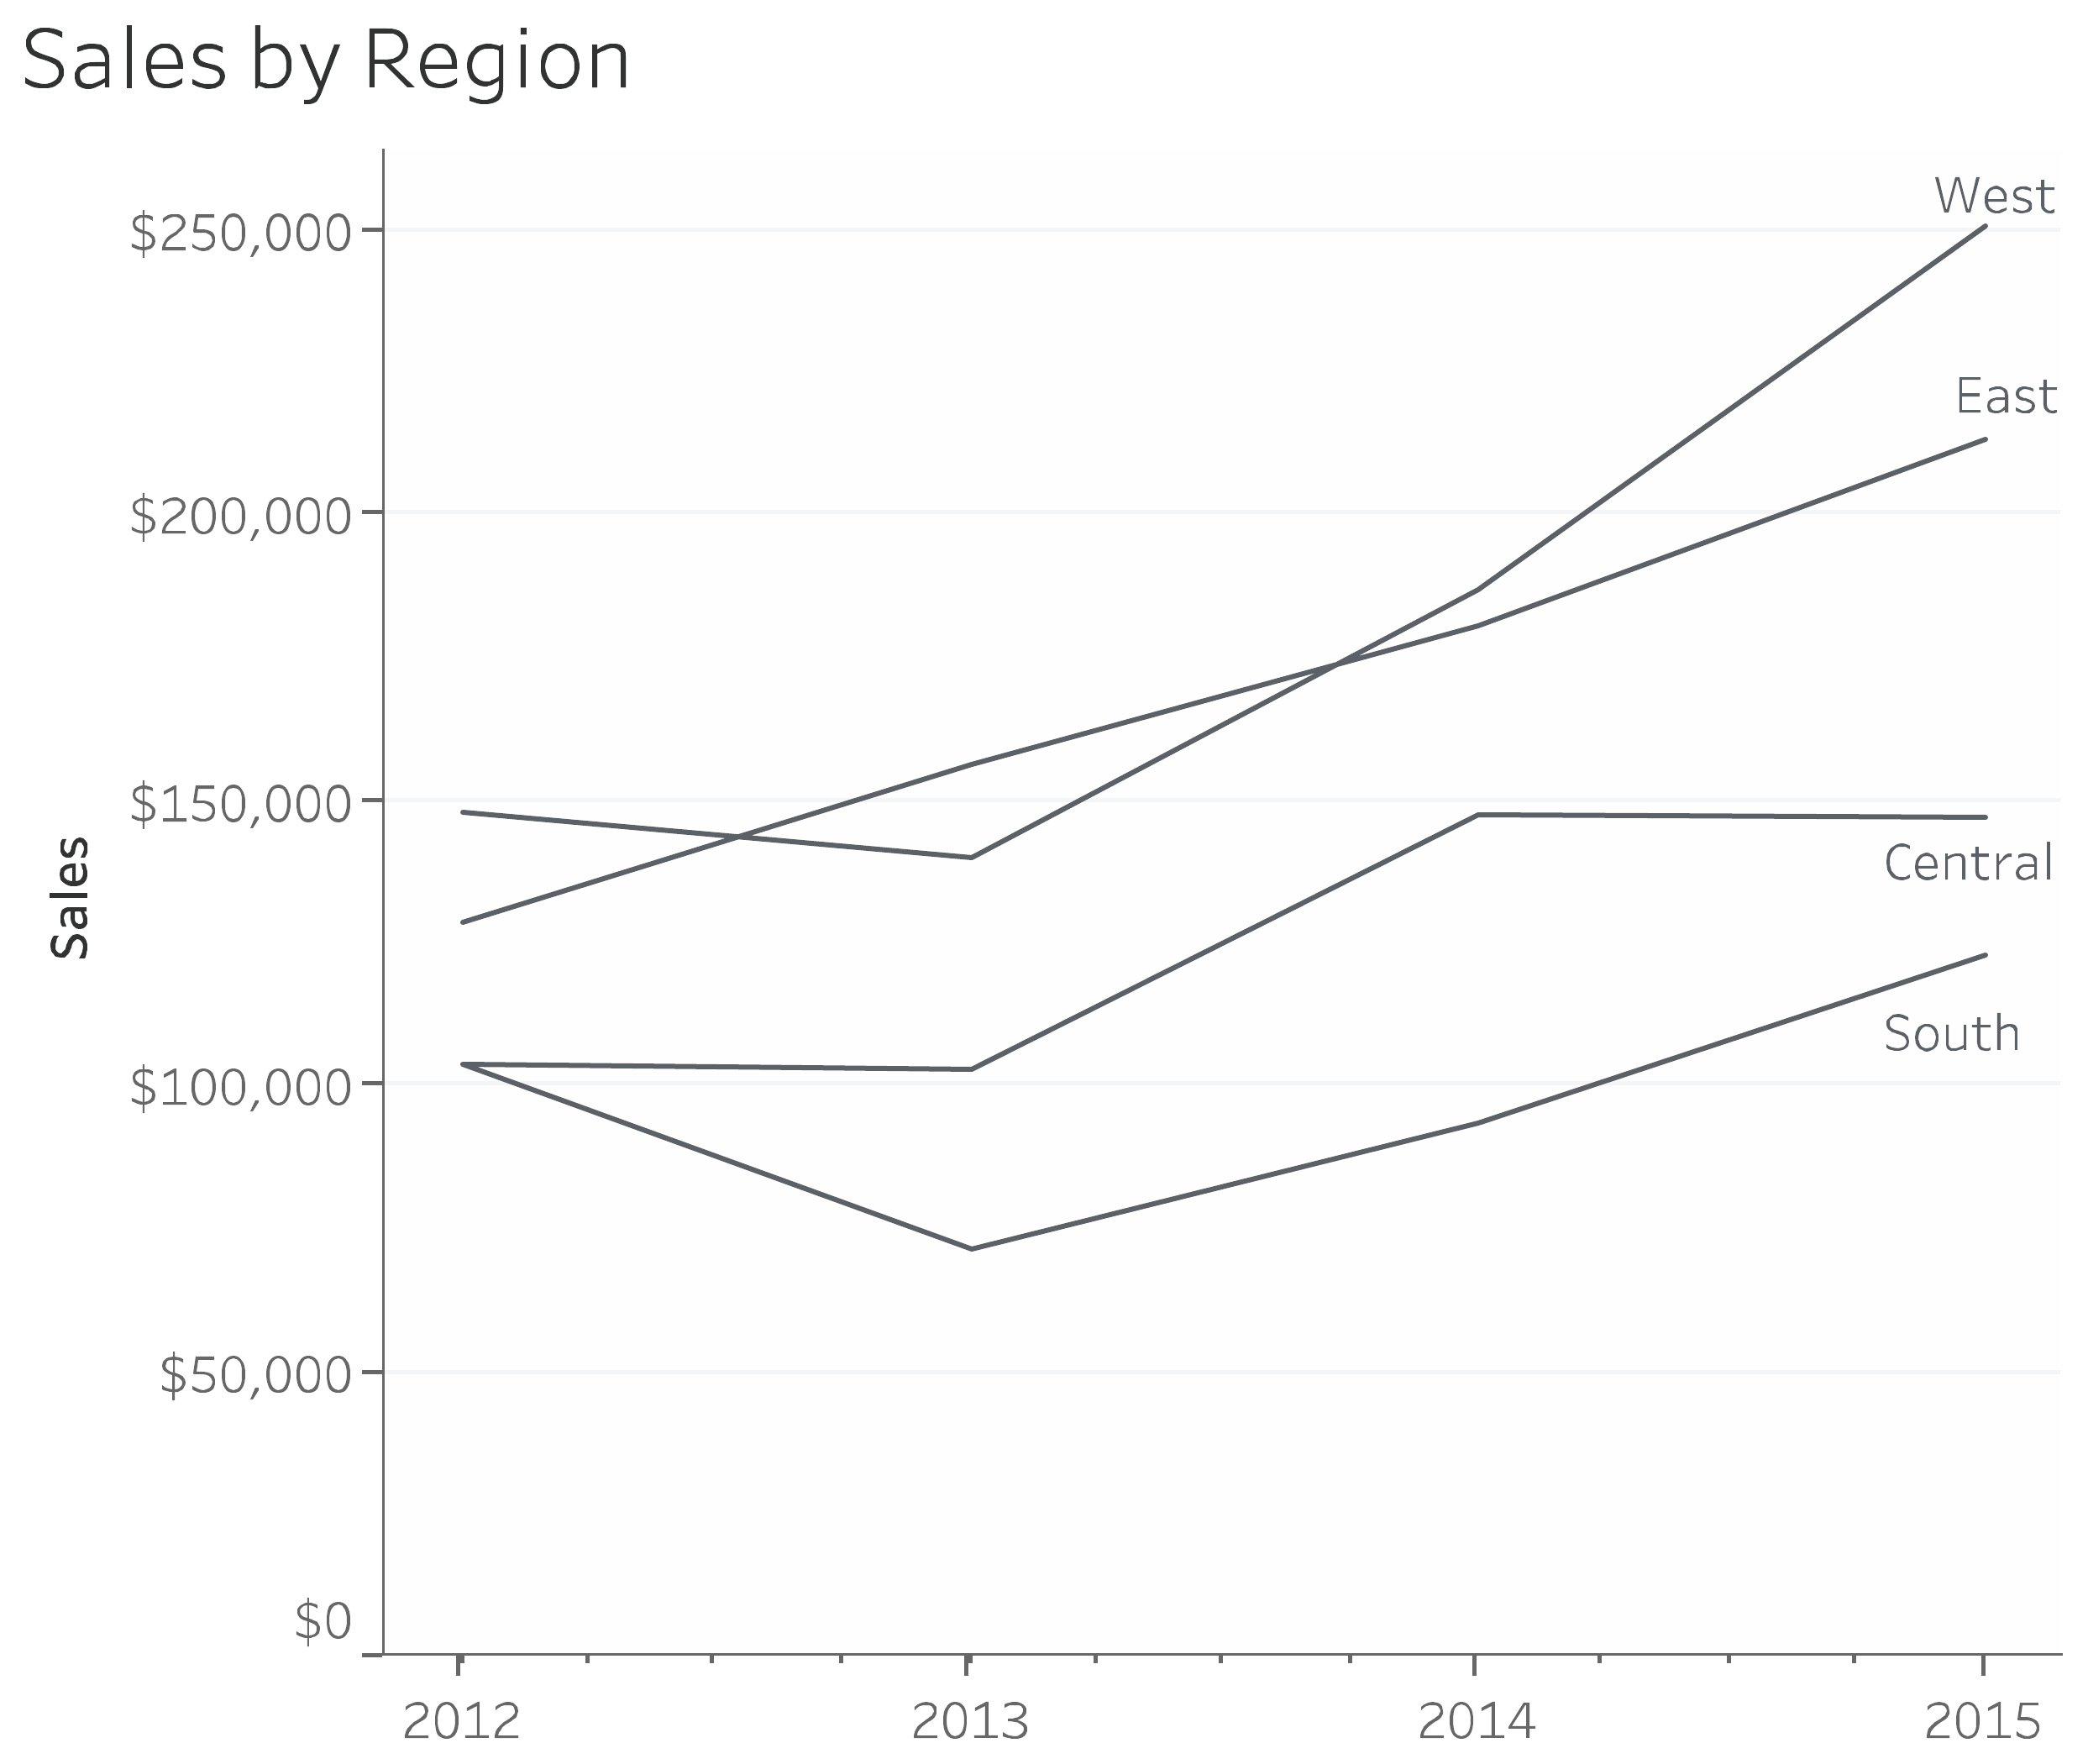
\includegraphics[width=\linewidth,height=0.49\textheight,keepaspectratio]{ch27_fig27_8_overlap_trim.png}
\end{center}
\footnotesize
\textbf{Problem:} overlapping lines are hard to trace when several regions cross in the same plot.
\end{column}
\begin{column}{0.49\textwidth}
\begin{center}
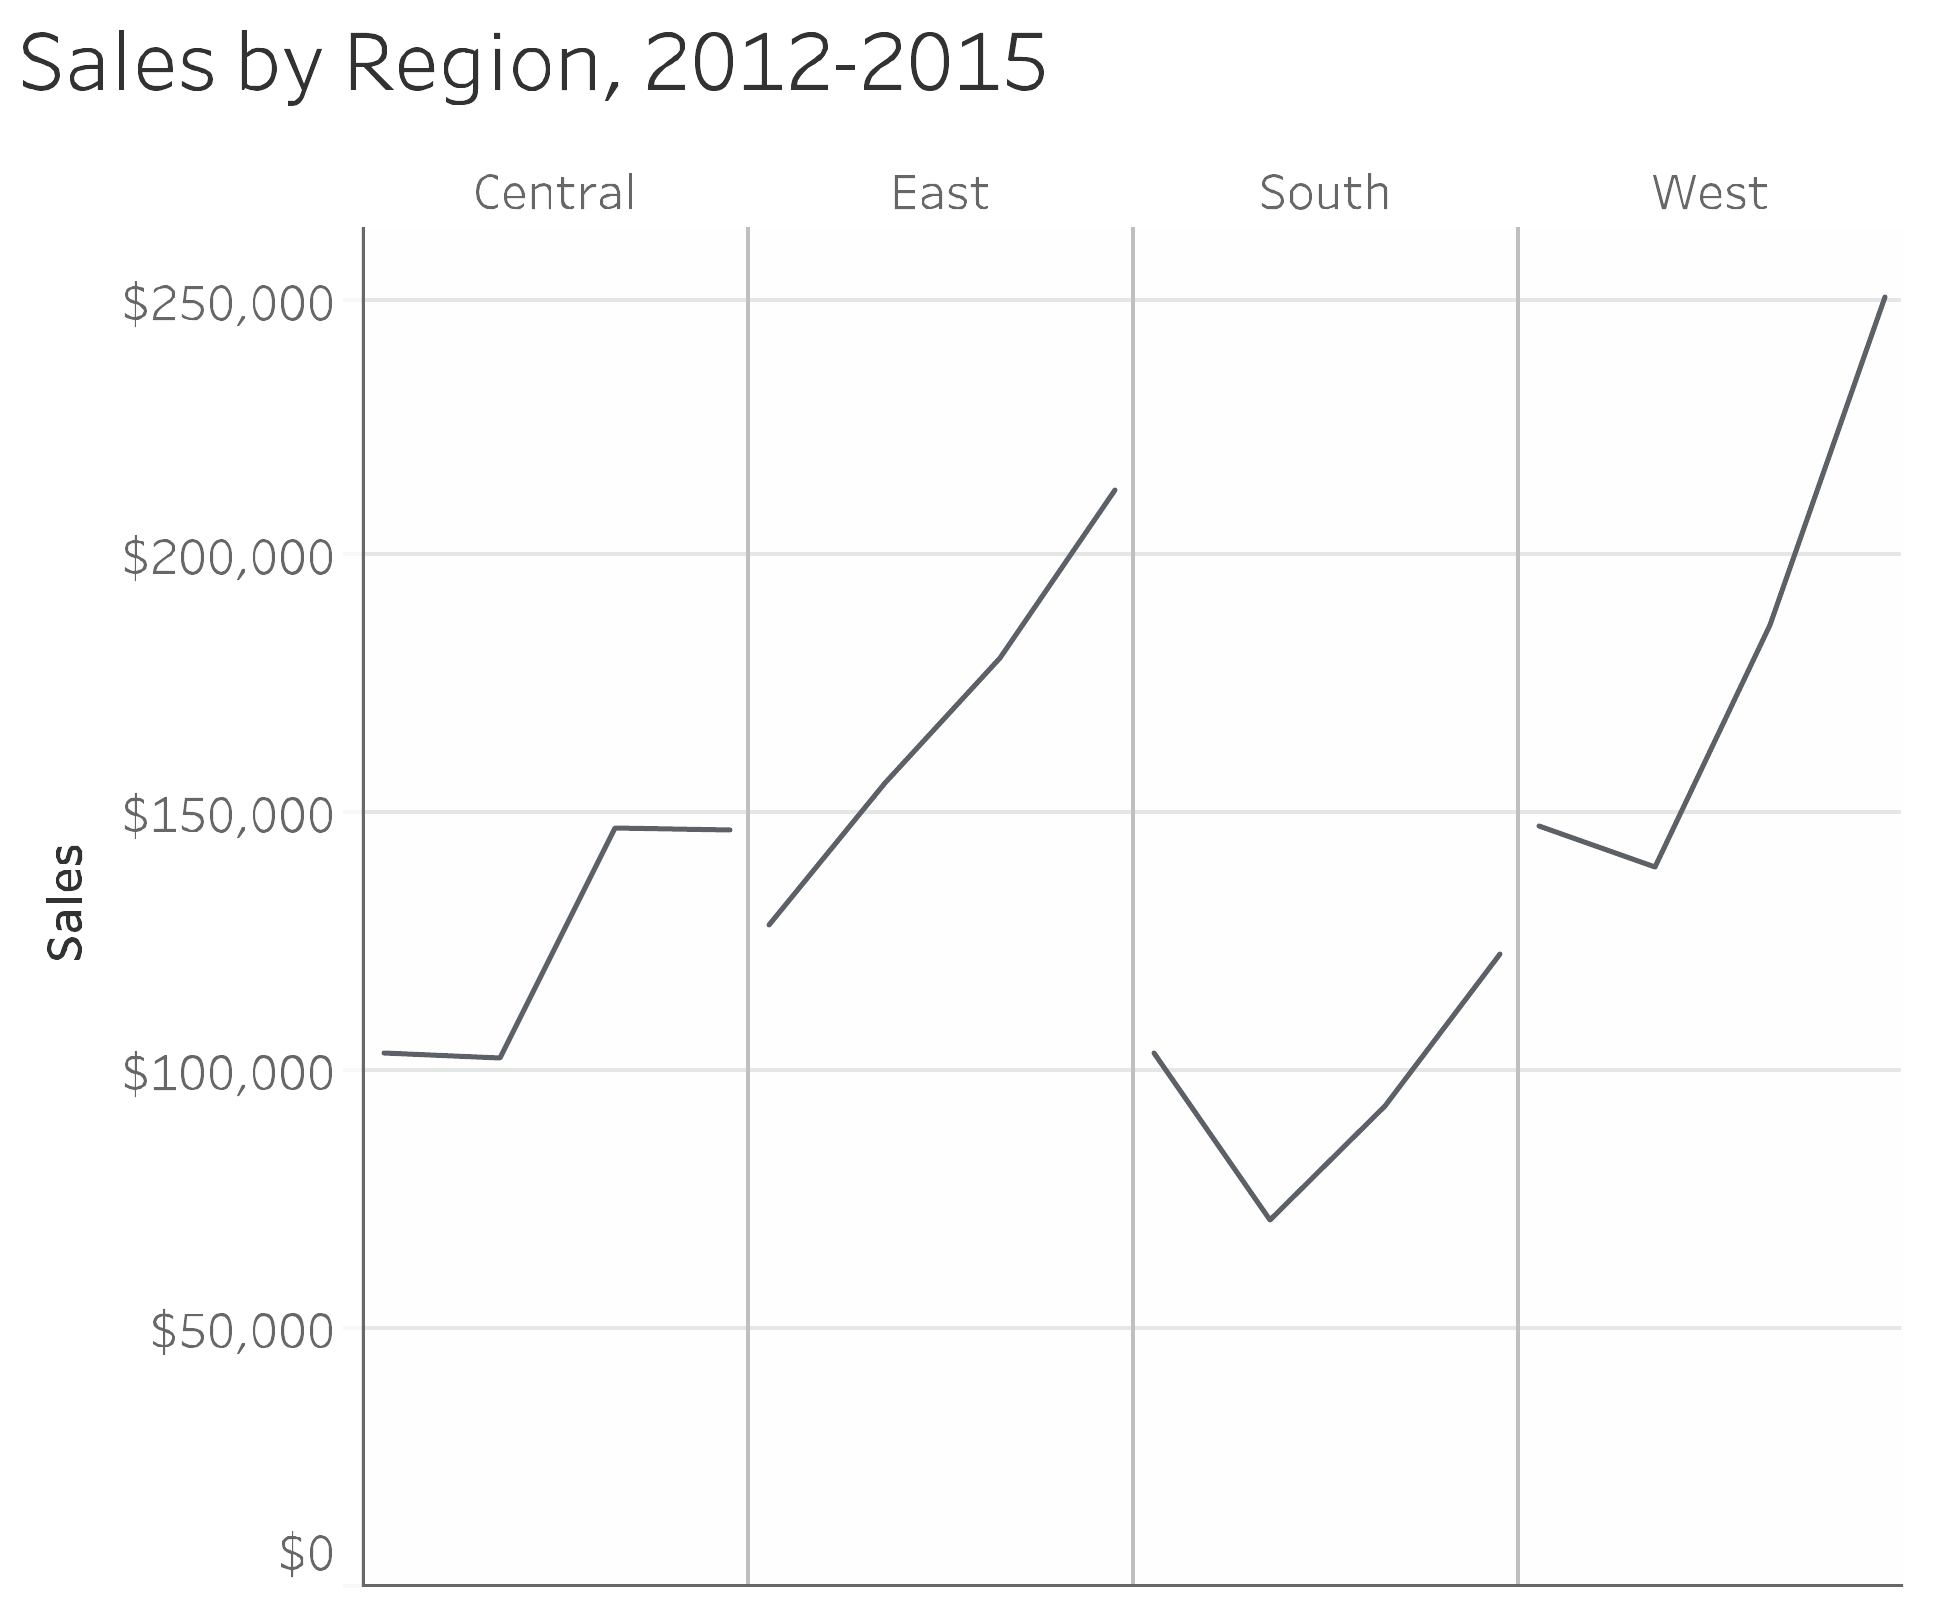
\includegraphics[width=\linewidth,height=0.49\textheight,keepaspectratio]{ch27_fig27_9_small_multiples.png}
\end{center}
\footnotesize
\textbf{Fix:} split dense series into small multiples so each region keeps a consistent time axis.
\end{column}
\end{columns}
\vspace{0.08cm}
\scriptsize\textbf{Other critiques:} red/green needs a non-color cue, and emphasis colors should be used sparingly.
\keymessage{Accessibility and line separation are design requirements, not cosmetic refinements.}
\end{frame}

% =========================================================
\begin{frame}{Conclusion}
\begin{block}{What Chapter 27 teaches}
\begin{itemize}
  \item A good dashboard helps decision-makers understand what is improving, what is worsening, and where action is needed.
  \item This dashboard succeeds because it follows three clear business goals.
  \item The three-row plus one-summary-column layout makes scanning fast.
  \item Small charts, direct labels, and limited color reduce clutter.
  \item The design still requires care with accessibility, overlapping lines, and chart consistency.
\end{itemize}
\end{block}
\keymessage{The goal is not more data on screen; it is faster decisions from the right evidence.}
\end{frame}

% =========================================================
\begin{frame}{References}
\footnotesize
\begin{itemize}
  \item Steve Wexler, Jeffrey Shaffer, Andy Cotgreave. \textit{The Big Book of Dashboards}, Chapter 27: Telecom Operator Executive Dashboard.
  \item Dundas Data Visualization sample dashboard: Telecom / Wireless Executive Strategy Dashboard.
  \item O'Reilly online excerpt for Chapter 27: \url{https://www.oreilly.com/library/view/the-big-book/9781119282716/c27.xhtml}
  \item Dashboard design references: related metric grouping, proximity, clutter reduction, clear KPI structure, and accessibility.
\end{itemize}
\vfill
\begin{center}
\Large\textcolor{cttBlue}{Thank you}
\end{center}
\end{frame}

\end{document}
